%\documentclass[10pt,a4paper,titlepage]{report}
\documentclass{report}

\usepackage{subcaption}
\usepackage[utf8]{inputenc}
\usepackage{amsmath}
\usepackage{amsthm}
\usepackage{amssymb}
\usepackage[linesnumbered,ruled]{algorithm2e}
\usepackage[usenames]{color}
\usepackage{float}
\usepackage{subfiles}
\usepackage{url}
\usepackage{nicefrac}
\usepackage{graphicx, rotating, subcaption}
\usepackage{tikz}

\usetikzlibrary{positioning}

% style for boxes in RP
\tikzstyle{box} = [draw=black, thick, outer sep=0pt, align=center]

% style for nodes in RP
\tikzstyle{rpn} = [circle, black, draw=black, fill=black, inner sep=0pt, minimum size=0.2cm]

\SetKwInput{KwInput}{Input}
\SetKwInput{KwOutput}{Output}
\DontPrintSemicolon

\begin{document}
\title{Scalable Nonparametric $L_1$ Density Estimation via Sparse Subtree Partitioning}
\author{Axel Sandstedt\\{\small Supervisor: Raazesh Sainudiin}}
\maketitle

\newpage
\abstract{We consider the construction of multivariate histogram estimators for any density $f$ seeking to minimize its $L_1$ distance to the true underlying density using arbitrarily large sample sizes.
Theory for such estimators exist and the early stages of distributed implementations are available. Our main contributions are
new algorithms which seek to optimise out unnecessary network communication taking place in the distributed stages of the construction of such estimators using sparse binary tree arithmetics.}
\newpage
\section*{Acknowledgments}
I wish to give my utmost gratitude to my supervisor Raazesh Sainudiin for his guidance within this multidisciplinary area. He gave me interesting problems to tackle
and in the process facilitated my learning of many valuable subjects and tools. He also pushed me in the right direction and kept the project coherent and on track.

\newpage
\tableofcontents
\newpage

\chapter*{Introduction}
The problem of density estimation may be approached in several different ways, with many methods assuming the existence of derivatives of the unknown density being estimated in order to achieve certain statistical properties. In this thesis we concern ourselves with 
the $L_1$-based density estimation method described in \cite{MDE}. The method is built upon the space partitioning structure of regular pavings and their properties, all found in \cite{Mapped Regular Pavings} and \cite{MDE}.
A quick summary of the method is that the support of the density can be partitioned using a binary space partitioning scheme and transformed into a $\mathbb{R}$-mapped regular paving, or $\mathbb{R}$-MRP for short, 
which is a mapping from the generated partition cells to $\mathbb{R}$. If the partitioning is done in such a way that some mathematical assumptions are satisfied, guarantees on the estimator can be made.

Improvements to the method was later made in \cite{Scalable Multivariate Histograms} by putting forward efficient encodings or labels for the partitions and distributed versions of some of its sub-problems. 
The latest improvements to the algorithmic properties of the method
can be found in \cite{Scalable Algorithms},  wherein the algorithms are approached
from a bottom-up perspective, that starts from a tree of the data points itself, instead of a top-down one, through a
sparse tree representation of the data and
rewrites the algorithms to suit this new setting. The method achieves its full potential when put in a distributed setting, as one of its goals is to handle very large amounts of data requiring 
more than one machine in order to be efficiently processed. Many stages of the method also lend themselves surprisingly well to the distributed setting.

The outline of this thesis is roughly as follows. We first formalize the setting by describing the $L_1$ setting and any assumptions made. 
Furthermore, some tools and definitions are needed in the $L_1$ setting which can be found in \cite{CMDE}. We also formalize data-dependent partitioning
and reiterate a consistency theorem for histogram estimators from \cite{Consistency}. Next we shall need to define mapped regular pavings
and some of their properties \cite{Mapped Regular Pavings}. Lastly, we need to go into the distributed setting and define efficient encodings, orderings and sparse representation of data structures given in
\cite{Scalable Multivariate Histograms} and \cite{Scalable Algorithms}, and then end the background by defining the minimum distance estimate in this context.
After the background has been given, we will describe a new approach to minimizing the communication cost within the algorithm called subtree partitioning in which we sort the data such that all points within certain
large subtrees will reside on the same machine, sharing many ideas with distributed sorting. 
A new way of doing distributed Scheffé set calculations is also given, in which no communication between machines
have to take place, and only a preprocessing step of sorting every machine's local data is needed.

We contribute, among other code optimisations, an implementation of these two ideas in the open-source Scala library found at \cite{SparkDensityTree}, which utilizes the distributed computation engine of Apache Spark.
At the end of the paper we provide timings, results, current limitations of the implementation, and directions for further work. The most interesting results involve the estimation of four distributions using 1 TB of data. See \cite{SparkDensityTreeExamples} for a detailed user guide with examples and applications
for how to use the library.

\chapter{Density Estimation}
\section{The $L_1$ setting}
We start by bringing forth some definitions and results found in \cite{CMDE} which we shall need later.
Consider a $\mathcal{B}(\mathbb{R})$-measurable random variable $\mathbf{X}:\Omega \rightarrow \mathbb{R}^d$
with density $f$ and suppose that $g : \mathbb{R}^d \rightarrow \mathbb{R}$ is some other density. The $L_1$ distance between $f$ and $g$ may be defined as
\begin{align*}
	\int_{\mathbb{R}^d} |f - g|.
\end{align*}
The distance has the nice property of being easily interpreted, and is connected to the total variation by Scheffé's Identity:
\begin{align*}
	\sup_{A \in \mathcal{B}(\mathbb{R}^d)} \ \bigg| \int_A f - \int_A g \ \bigg| = \frac{1}{2}\int_{\mathbb{R}^d} |f - g|.
\end{align*}
Suppose that $X_1,\dots,X_n \overset{\text{i.i.d}}{\sim} X$ and let $f$ denote the density of $X$. A natural thing to do in many applications is to estimate $f$.
Depending on the construction of the estimate, one may be able to sample from the density estimate, or use the estimate in regression analysis and so on. The estimator
\begin{align*}
	f_n(x; X_1,\dots,X_n) : \mathbb{R}^d \times \big(\mathbb{R}^d\big)^n \rightarrow \mathbb{R}
\end{align*}
is said to have \textit{universal performance guarantees} if it achieves certain desirable properties \cite{CMDE} that hold for any underlying density $f$. Thus, when working in such contexts, we 
are within the most general framework of density estimation where we are only assuming that our sample comes from some continuous distribution $f \in L_1$. 
\newpage
What is of interest to us is the construction of an efficient
estimator $f_n$ in the computational sense and deriving a universal upper bound on the expected $L_1$ distance to $f$.
We say that the estimator $f_n$ is \textit{additive} if for some measurable function $K : \mathbb{R}^d \times \mathbb{R}^d \rightarrow \mathbb{R}$, $f_n$ can be written in the form
\begin{align*}
	f_n = \frac{1}{n}\sum_{i=1}^n K(x; X_i).
\end{align*}
Any such $f_n$ is called \textit{regular} if $\forall x : \mathbb{E}|K(x;X)| < \infty$. Consider a multivariate density histogram $h_n$ with a finite number 
of non-intersecting and non-empty cells with finite volume $P_1,\dots,P_m$. The density may be written as 
\begin{align*}
	h_n(x;X_1,\dots,X_n) = \frac{1}{n}\sum_{i=1}^{n} \sum_{j = 1}^{m} \frac{\mathbb{I}_{[x\in P_j]}\mathbb{I}_{[X_i\in P_j]}}{\text{volume}(P_j)} = \frac{1}{n}\sum_{i=1}^{n} K(x;X_i).
\end{align*}
Since $K$ is the sum of a finite number of measurable functions, we conclude that $h_n$ is additive. Regularity follows from observing that for any $x \in \mathbb{R}^d$, the following holds:
\begin{align*}
|K(x;X)| \leq \underset{j\leq m}{\text{max }} \frac{1}{\text{volume}(P_j)}.
\end{align*}

For an i.i.d sample $(X_1,\dots,X_n)$ we define the \textit{empirical measure} $\mu_n$ as 
\begin{align*}
	\mu_n(A) := \mu_n(A; X_1,\dots,X_n) := \frac{1}{n}\sum_{i = 1}^n \mathbb{I}_{[X_i \in A]},
\end{align*}


\section{Yatracos Classes and the Minimum Distance Estimate}
Consider two densities $f_{n,\theta}, f_{n,\omega} : \mathbb{R}^d \rightarrow \mathbb{R}$. We define a \textit{Scheffé set} as the set
\begin{align*}
	A(f_{n,\theta},f_{n,\omega}) := \{x : f_{n,\theta}(x) > f_{n,\omega}(x)\}.
\end{align*}
Now, suppose that we have a finite set of estimate indices $\theta \in \Theta$. The set of all distinct Scheffé sets of $\Theta$ is denoted by
\begin{align*}
	\mathcal{A}_\Theta := \{A_{f_{n,\theta}, f_{n,\omega}} :  \theta \neq \omega\}
\end{align*}
and is known as the \textit{Yatracos class} of $\Theta$. Furthermore, assume that for any $\theta \in \Theta$, $f_{n,\theta}$ represents an estimate of some unknown but fixed density $f$.
Define $\Delta_\theta$ as the supremum of the absolute distance between $f_{n,\theta}$ and $\mu_n$ over $\mathcal{A}_\Theta$:
\begin{align*}
	\Delta_\theta := \sup_{A \in \mathcal{A}_\Theta} \bigg| \int_A f_{n,\theta} - \mu_n(A) \bigg|.
\end{align*}
The \textit{minimum distance estimate} $\psi_n$ (MDE) within the set of estimators in $\Theta$ generating $\mathcal{A}_\Theta$ is defined to be the estimate minimising 
the above distance:
\begin{align*}
	\psi_n := f_k,\quad k = \min \underset{i \in {1,\dots,m}}{\text{argmin }} \Delta_i.
\end{align*}
If several estimates obtain the minimum, we define the MDE to be the estimate with the smallest index. However, since there is a dependence on $X_1,\dots,X_n$ for both
the empirical measure and any created estimators, we run the risk of choosing degenerate estimators as the MDE.  (\cite{CMDE}, Section 10.1) proposes a hold-out method in 
which a fraction $\varphi \in (0,\frac{1}{2})$ of the original sample is reserved for a validation set to compute the empirical measure $\mu_{\lfloor\varphi n\rfloor}$ over, 
and the rest are assigned to the training set used in the construction of any estimators $f_{n-\lfloor\varphi n\rfloor, \theta}$.

\section{Shatter Coefficients and Vapnik-Chervonekis dimensions}
We shall need some more tools to formally deal with partitions of $\mathbb{R}^d$. Let $\mathcal{A}$ denote a class of subsets $A \subseteq \mathbb{R}^d$. We let $\mathcal{S}_\mathcal{A}(n)$
denote the \textit{shattering coefficient} of $\mathcal{A}$ depending on $n$, and it is defined by
\begin{align*}
	\mathcal{S}_\mathcal{A}(n) := \max_{(x_1,\dots,x_n) \in (\mathbb{R}^d)^n} \big|\{A \cap \{x_1,\dots,x_n\} : A \in \mathcal{A}\}\big|.
\end{align*}
Intuitively, $\mathcal{S}_\mathcal{A}(n)$ describes the largest amount of unique ways the class could shatter or split a set of $n$ points residing in $\mathbb{R}^d$. 
The \textit{Vapnik-Chervonenkis dimension} $V_\mathcal{A}$ of $\mathcal{A}$ is defined as the largest integer $n$ such that $\mathcal{S}_\mathcal{A}(n) = 2^n$. Thus
$V_\mathcal{A}$ represents the largest number of points which $\mathcal{A}$ can fully shatter. Vapnik and Chervonenkis (1971) provided the following theorem which relates
shattering coefficients to an i.i.d sample $(X_1,\dots,X_n)$ coming from a distribution $\mu$ and its corresponding empirical measure:\newline

\noindent\textbf{(\cite{Pattern}, Theorem 12.5): } Given a class of sets $\mathcal{A}$, a sample $(X_1,\dots,X_n)$ with common probability distribution $\mu$ and any $\epsilon > 0$, the
following inequality holds:
\begin{align*}
	\mathbb{P}\bigg( \underset{A \in \mathcal{A}}{\text{sup}} \big|\mu_n(A) - \mu(A)\big| > \epsilon \bigg) \leq 8 S_\mathcal{A}(n) e^{-n\epsilon^2/32}.
\end{align*}

\section{Partitions and Partition Schemes}
In this section we reiterate on topics found in \cite{Consistency} and gain some intuition regarding histograms based upon data-driven partitions. 
The paper provides definitions and an important $L_1$ consistency theorem which can be used in proving $L_1$ consistency of the estimator
we shall later consider. 
\newpage
Let $\pi$ denote a finite collection of non-intersecting $\mathcal{B}(\mathbb{R}^d)$-measurable subsets $A \subseteq \mathbb{R}^d$ such that $\bigcup_{A \in \pi} A = \mathbb{R}^d$.
We are interested in the properties of certain families of partitions, and as such let $\mathcal{A}$ denote any family of possibly infinitely many partitions $\pi$. Furthermore, let
\begin{align*}
	m(\mathcal{A}) := \underset{\pi \in \mathcal{A}}{\text{sup}}|\pi|
\end{align*}
denote the supremum over $\mathcal{A}$ with respect to the number of cells of any $\pi$. We define and measure the complexity of $\mathcal{A}$ 
by its ability to split a number of points; let $x_1,\dots,x_n \in \mathbb{R}^d$ and $B = \{x_1,\dots,x_n\}$. We define $\Delta(\mathcal{A},B)$ as the number of unique ways $\mathcal{A}$'s
partitions may split $B$:
\begin{align*}
	\Delta(\mathcal{A},B) := \big| \{ \{A_1 \cap B, \dots, A_r \cap B\} : \pi = \{A_1,\dots,A_r\} \in \mathcal{A} \} \big|.
\end{align*}
The \textit{growth function} of $\mathcal{A}$ is defined as 
\begin{align*}
	\Delta^*(\mathcal{A},n) := \max_{B = \{x_1,\dots,x_n\} \subset \mathbb{R}^d} \Delta(\mathcal{A},B).
\end{align*}
In the context of histogram estimators whose cells depend on the data, if we view the rules for constructing cells as fixed and $\mathcal{A}$ as the family of
possible partitions $\pi$ constructed using the rules, $\Delta^*(\mathcal{A},n)$ measures in some sense the estimator's reliance on individual points versus a set of points,
and is therefore of importance. This can in turn be related to the usual smoothing problem in which one chooses some bandwidth which affects how an estimator at any
point $x \in \mathbb{R}^d$ relies on nearby sample points. The following lemma bridges the concept of growth functions and
the empirical measure's performance over $\mathcal{A}$.\newline

\noindent\textbf{(\cite{Consistency}, Lemma 1): }Let $\mathcal{A}$ be any family of partitions of $\mathbb{R}^d$. Let $\epsilon > 0$ and $n \geq 1$. Then the following holds:
\begin{align*}
	\mathbb{P}\bigg( \underset{\pi \in \mathcal{A}}{\text{sup}}\sum_{A \in \pi} \big|\mu_n(A) - \mu(A)\big| > \epsilon \bigg) \leq 4 \Delta^*(\mathcal{A}, 2n)2^{m(\mathcal{A})} e^{-n\epsilon^2/32}.
\end{align*}
A corollary of this is that, for a given a sequence of i.i.d vectors $X_1,X_2,\dots$ with common distribution $\mu$ 
 and a sequence of partition families $\mathcal{A}_1,\mathcal{A}_2,\dots$, if we put certain limitations on how quickly
the two sequences $\{\Delta^*(\mathcal{A}_n,n)\}_{n=1}^\infty$ and $\{m(\mathcal{A}_n)\}_{n=1}^\infty$ are allowed to grow, then we can ensure almost sure convergence of the empirical measure $\mu_n$ to $\mu$
over $\mathcal{A}_n$:\newline

\noindent\textbf{(\cite{Consistency}, Corollary 1): }Consider the setup described above. As $n \rightarrow \infty$, if $n^{-1}m(\mathcal{A}_n) \rightarrow 0$ and
$n^{-1}\text{ln}(\Delta^*(\mathcal{A}_n,n))) \rightarrow 0$, then it is true that
\begin{align*}
	\mathbb{P}\bigg( \underset{n \rightarrow \infty}{\text{lim}}
	\underset{\pi \in \mathcal{A}}{\text{sup}}\sum_{A \in \pi} \big|\mu_n(A) - \mu(A)\big| = 0 \bigg) = 1.
\end{align*}

\noindent\textbf{Proof:}\quad The proof relies on an application of (\cite{Consistency}, Lemma 1) and the first Borel-Cantelli Lemma (\cite{Martingales}, Lemma 2.7).
Suppose that $\epsilon > 0$ and let $E_n$ denote the following event
\begin{align*}
	E_n := \big\{\omega : \underset{\pi \in \mathcal{A}}{\text{sup}}\sum_{A \in \pi} \big|\mu_n(A) - \mu(A)\big| > \epsilon \big\}.
\end{align*}
By (\cite{Consistency}, Lemma 1) we have that
\begin{align*}
	\sum_{n=1}^\infty \mathbb{P}(E_n) &\leq  \sum_{n=1}^\infty 4\Delta^*(\mathcal{A}_n, 2n)2^{m(\mathcal{A}_n)} e^{-n\epsilon^2/32} \\
					  &= \sum_{n=1}^\infty e^{\text{ln}(4) + \text{ln}\big(\Delta^*(\mathcal{A}_n, 2n)\big) + {m(\mathcal{A}_n)}\text{ln}(2)  -n\epsilon^2/32} \\
					  &= \sum_{n=1}^\infty \bigg(e^{n^{-1}\text{ln}(4) + n^{-1}\text{ln}\big(\Delta^*(\mathcal{A}_n, 2n)\big) + n^{-1}{m(\mathcal{A}_n)}\text{ln}(2)  -\epsilon^2/32}\bigg)^n \\
\end{align*}
Suppose that $x^{2n} = \{x_1,\dots,x_{2n}\}$ maximises $\Delta(\mathcal{A}_n, x^{2n})$ such that $\Delta(\mathcal{A}_n, x^{2n}) = \Delta^*(\mathcal{A}_n, 2n)$.
Let $\mathcal{C}$ consist of sets produced when splitting $x_1,\dots,x_n$ over $\mathcal{A}_n$,
and similarly $\mathcal{D}$ when splitting $x_{n+1},\dots,x_{2n}$. 
When splitting $x^{2n}$ over some partition of $\mathcal{A}_n$ and generating a set $B$, there exists sets $C = \{C_1,\dots,C_r\} \in \mathcal{C}$ and $D = \{D_1,\dots,D_r\} \in \mathcal{D}$ such that 
\begin{align*}
	B = \{C_1 \cup D_1, \dots, C_r \cup D_r\}
\end{align*}
we can thus define a mapping from $\mathcal{C}\times\mathcal{D}$ onto the set of generated sets made from splitting $x^{2n}$. It follows that 
\begin{align*}
	\Delta^*(\mathcal{A}_n, 2n) \leq |\mathcal{C}||\mathcal{D}| \leq \Delta^*(\mathcal{A}_n, n)^2.
\end{align*}
Consequently, together with the convergence assumptions from the start, we get 
\begin{align*}
	&n^{-1}\text{ln}(4) + n^{-1}\text{ln}\big(\Delta^*(\mathcal{A}_n, 2n)\big) + n^{-1}{m(\mathcal{A}_n)}\text{ln}(2) \\
	&\leq n^{-1}\text{ln}(4) + 2n^{-1}\text{ln}\big(\Delta^*(\mathcal{A}_n, n)\big) + n^{-1}{m(\mathcal{A}_n)}\text{ln}(2) \rightarrow 0
\end{align*}
This implies that, together with $e^x$ being continuous and monotonically increasing, the sum of probabilities is bounded from above by a constant plus some bounded geometric series.
By the first Borel-Cantelli Lemma it follows that 
\begin{align*}
	\mathbb{P}\big(\text{lim sup} \ E_n \big) = 0.
\end{align*}
Since $\epsilon > 0$ was arbitrarily set, we conclude that 
\begin{align*}
	\mathbb{P}\bigg( \underset{n \rightarrow \infty}{\text{lim}}
	\underset{\pi \in \mathcal{A}}{\text{sup}}\sum_{A \in \pi} \big|\mu_n(A) - \mu(A)\big| = 0 \bigg) = 1.
\end{align*}

\hfill$\square$

\noindent \newline
We now wish to formally present the previous histogram context we touched upon. Define a \textit{n-sample partitioning rule} $\pi_n$ to be a 
mapping from $(\mathbb{R}^d)^n$ to the set of partitions consisting of Borel-measurable sets $A \subseteq \mathbb{R}^d$. Consider a sample of i.i.d random vectors $(X_1,\dots,X_n)$.
We may define a histogram estimator $f_n$ using partitioning rule $\pi_n$ as follows:
\begin{align*}
	f_n(x) := \sum_{\textrm{\shortstack{$A \in \pi_n(X_1,\dots,X_n)$\\\text{volume}$(A) < \infty$}}} \frac{\sum_{i=1}^n \mathbb{I}_A(X_i)}{n \cdot \text{volume}(A)}\mathbb{I}_{A}(x).
\end{align*}
Note that the estimator need not necessarily be a density.

In order to consider all sample sizes, we define a \textit{partitioning scheme} $\Pi = \{\pi_n\}_{n=1}^\infty$ to be a sequence of partitioning rules,
one for every sample size. Note that the rules are deterministic and the randomness comes from the sample. Thus we say that such histograms are data-driven or adaptive, since its
partitioning is based on the realised sample.
Since $\Pi$ is a sequence of mappings $\pi_n$, we may associate $\Pi$ with the sequence $\{\mathcal{A}_n\}_{n=1}^\infty$ of families where $\mathcal{A}_n$ denotes the family of partitions
\begin{align*}
	\mathcal{A}_n := \{\pi_n(x_1,\dots,x_n) : x_1,\dots,x_n \in \mathbb{R}^d \}.
\end{align*}
The last definition we shall need is the notion of a set's diameter. If $A \subseteq \mathbb{R}^d$ then we define the diameter of $A$ to be 
\begin{align*}
	\text{diam}(A) := \underset{x,y\in A}{\text{sup}}||x-y||.
\end{align*}
We can now state the consistency theorem.\newline

\noindent\textbf{(\cite{Consistency}, Theorem 1):} Let $\{X_n\}_{n=1}^\infty$ be a i.i.d sequence of random vectors with common distribution $X \sim \mu$ and density $f$. Consider a fixed partitioning scheme
$\Pi = \{\pi_n\}_{n=1}^\infty$ and let $f_n$ denote the estimator defined as above.
Suppose that for the sequence of families $\{\mathcal{A}_n\}_{n=1}^\infty$ associated with $\Pi$, it is true that (a) $n^{-1}m(\mathcal{A}_n) \rightarrow 0$ and 
(b) $n^{-1}\text{ln}(\Delta^*(\mathcal{A}_n, n)) \rightarrow 0$. 
Furthermore, consider the conditional probability $\mu\big(A^\lambda| X_1,\dots,X_n \big)$, where 
\begin{align*}
	A^\lambda := \{x : x \text{ resides in a cell of diameter greater than }\lambda \},
\end{align*}
and suppose that (c) for any $\lambda > 0$, the following holds:
\begin{align*}
	\mathbb{P}\big(\lim_{n \rightarrow \infty} \mu(A^\lambda | X_1,\dots,X_n)  \big) = 0.
\end{align*}
Then $f_n$ is asymptotically consistent in $L_1$, i.e.  
\begin{align*}
	\mathbb{P}\big( \lim_{n \rightarrow \infty} \int \big| f(x) - f_n(x) \big|dx = 0 \big) = 1.
\end{align*}
\newline\noindent We have thus defined the requirements for a histogram estimator to be asymptotically consistent. We note that the theorem does not state anything about any special partition shapes, 
and only requires certain probability and complexity criteria on the partitioning scheme fulfilled.

\chapter{Regular Pavings}
In this Section we define the mathematical structure of regular pavings which form the basis for our estimator's partitioning scheme. After the structure has been introduced, we can define the estimator and the strategies for finding them.
\section{Regular Pavings}
A \textit{regular paving} (RP) $\rho$ describes a recursive mathematical structure which is defined by a $d$-dimensional root box, or hyperrectangle:
\begin{align*}
	\mathbf{x}_{\rho} = [x_{1,\text{low}}, x_{1,\text{high}}] \times \cdots \times [x_{d,\text{low}}, x_{d,\text{high}}],
\end{align*}
and a sequence of splits applied to it. Splitting the root box is fully deterministic; the axis to split is defined by:
\begin{align*}
	\text{axis} := \min \ \underset{\iota = 1,\dots,d}{\operatorname{argmax}} \  x_{\iota,\text{high}} - x_{\iota,\text{low}}.
\end{align*}
Thus we split the regular paving in the first dimension in which the box's side achieves the maximum length. Suppose a split happens along dimension $\iota$. Then two new RPs $\rho\sf{L}$ and $\rho\sf{R}$ are created,
with respective root boxes
\begin{align*}
	\mathbf{x}_{\rho\sf{L}} &:= [x_{1,\text{low}}, x_{1,\text{high}}] \times \cdots \times [x_{\iota,\text{low}}, x_{\iota,\text{mid}(\mathbf{x}_\iota)}\ ) \times \cdots \times [x_{d,\text{low}}, x_{d,\text{high}}], \\
	\mathbf{x}_{\rho\sf{R}} &:= [x_{1,\text{low}}, x_{1,\text{high}}] \times \cdots \times [x_{\iota,\text{mid}(\mathbf{x}_\iota)}, x_{\iota,\text{high}}] \times \cdots \times [x_{d,\text{low}}, x_{d,\text{high}}].
\end{align*}
where the function \text{mid} refers to the midpoint of $\mathbf{x}_\iota = [x_{\iota,\text{low}}, x_{\iota,\text{high}}]$. If $\mathbf{x}_\rho$ is not closed, it may be closed again by taking the hull
of itself and from there apply the above operations.  It is useful to assign labels to each new RP
produced from the split of a RP $\rho$. If we consider the two cells above, $\mathbf{x}_{\rho \sf{L}}$ and $\mathbf{x}_{\rho \sf{R}}$, their respective 
RPs may be assigned labels $\rho \sf{L}$ and $\rho \sf{R}$. In this view, each RP may be viewed as a binary tree, where the leaves of the tree represents a set of disjoint cells whose union is exactly the original root box. 

We provide an example from \cite{Mapped Regular Pavings}. The root box $\mathbf{x}_\rho$ under consideration is represented as the root node in a binary tree, labelled $\rho$. The first split is along the left-right
axis, and as both sides are of equivalent length, we conclude that the left-right dimension comes before the up-down dimension. Also note that every split of a box results in two equivalently sized sub-boxes.
This follows from the splitting rule always slicing a side in the middle, which, together with the deterministic choice of splitting axis, implies that any two equivalent binary trees representing the same root box will
represent equivalent RPs.

\begin{figure}[H]
  \begin{center}
    \scalebox{0.55}{
      \setlength{\unitlength}{5cm}
      \begin{picture}(6, 1.7)(0,0)
        %root box
        \put(0.375, 1.175){\circle*{0.08}}
        \put(0.373,1.255){$\rho$}
        \put(0,0){\line(0,1){0.75}}  %vertical line
        \put(0,0){\line(1,0){0.75}}  %horizontal line
        \put(0.75,0){\line(0,1){0.75}} %vertical line
        \put(0,0.75){\line(1,0){0.75}} %horizontal line
	\put(0.35, 0.35){\Large{$\mathbf{x}_\rho$}}
        %XL and XR
        \put(1.275, 1.3){\circle*{0.08}}
        \put(1.273,1.38){$\rho$}
        \put(1.075, 1.1){\circle*{0.08}}
        \put(1.05,0.975){$\rho \sf{L}$}
        \put(1.475, 1.1){\circle*{0.08}}
        \put(1.45,0.975){$\rho \sf{R}$}
        \put(1.275, 1.3){\line(-1,-1){0.2}}
        \put(1.275, 1.3){\line(1,-1){0.2}}
        \put(0.9,0){\line(0,1){0.75}}  %vertical line
        \put(0.9,0){\line(1,0){0.75}}  %horizontal line
        \put(1.65,0){\line(0,1){0.75}} %vertical line
        \put(0.9,0.75){\line(1,0){0.75}} %horizontal line
        \put(1.275,0){\line(0,1){0.75}} %vertical line
	\put(1.0, 0.35){\Large{$\mathbf{x}_{\rho \mathsf{L}}$}}
	\put(1.4, 0.35){\Large{$\mathbf{x}_{\rho \mathsf{R}}$}}
        %XLL, XLR, XR
        \put(2.275, 1.425){\circle*{0.08}} %rho
        \put(2.273,1.5){$\rho$}
        \put(2.275, 1.425){\line(-1,-1){0.2}}
        \put(2.075, 1.225){\circle*{0.08}} %L
        \put(2.075, 1.225){\line(-1,-1){0.2}}
        \put(1.875, 1.025){\circle*{0.08}} %LL
        \put(1.83,0.9){$\rho \sf{LL}$}
        \put(2.075, 1.225){\line(1,-1){0.2}}
        \put(2.275, 1.025){\circle*{0.08}} %LR
        \put(2.25,0.9){$\rho \sf{LR}$}
        \put(2.275, 1.425){\line(1,-1){0.2}}
        \put(2.475, 1.225){\circle*{0.08}} %R
        \put(2.46,1.1){$\rho \sf{R}$}
        \put(1.8,0){\line(0,1){0.75}}  %vertical line
        \put(1.8,0){\line(1,0){0.75}}  %horizontal line
        \put(2.55,0){\line(0,1){0.75}} %vertical line
        \put(1.8,0.75){\line(1,0){0.75}} %horizontal line
        \put(2.175,0){\line(0,1){0.75}} %vertical line
        \put(1.8,0.375){\line(1,0){0.375}} %horizontal line
	\put(1.915, 0.545){\Large{$\mathbf{x}_{\rho \mathsf{LR}}$}}
	\put(1.915, 0.15){\Large{$\mathbf{x}_{\rho \mathsf{LL}}$}}
	\put(2.3, 0.35){\Large{$\mathbf{x}_{\rho \mathsf{R}}$}}
        %XLL, XLR, XRL, XRR
        \put(3.075, 1.425){\circle*{0.08}} %rho
        \put(3.073,1.5){$\rho$}
        \put(3.075, 1.425){\line(-1,-1){0.2}}
        \put(2.875, 1.225){\circle*{0.08}} %L
        \put(2.875, 1.225){\line(-1,-1){0.2}}
        \put(2.675, 1.025){\circle*{0.08}} %LL
        \put(2.64,0.9){$\rho \mathsf{LL}$}
        \put(2.875, 1.225){\line(1,-1){0.2}}
        \put(3.075, 1.025){\circle*{0.08}} %LR
        \put(3.0,0.9){$\rho \sf{LR}$}
        \put(3.075, 1.425){\line(1,-1){0.2}}
        \put(3.275, 1.225){\circle*{0.08}} %R
        \put(3.175, 1.025){\circle*{0.08}} %RL
        \put(3.15,0.9){$\rho \mathsf{RL}$}
        \put(3.275, 1.225){\line(1,-1){0.2}}
        \put(3.475, 1.025){\circle*{0.08}} %RR
        \put(3.45,0.9){$\rho \sf{RR}$}
        \put(3.275, 1.225){\line(-1,-2){0.1}}
        \put(2.7,0){\line(0,1){0.75}}  %vertical line
        \put(2.7,0){\line(1,0){0.75}}  %horizontal line
        \put(3.45,0){\line(0,1){0.75}} %vertical line
        \put(2.7,0.75){\line(1,0){0.75}} %horizontal line
        \put(3.075,0){\line(0,1){0.75}} %vertical line
        \put(2.7,0.375){\line(1,0){0.75}} %horizontal line
	\put(2.8, 0.545){\Large{$\mathbf{x}_{\rho \mathsf{LR}}$}}
	\put(2.8, 0.15){\Large{$\mathbf{x}_{\rho \mathsf{LL}}$}}
	\put(3.15, 0.15){\Large{$\mathbf{x}_{\rho \mathsf{RL}}$}}
	\put(3.15, 0.545){\Large{$\mathbf{x}_{\rho \mathsf{RR}}$}}
        %XLL, XLLL, XLRL, XLRR, XRL, XRR
        \put(3.975, 1.55){\circle*{0.08}} %rho
        \put(3.973,1.65){$\rho$}
        \put(3.975, 1.55){\line(-1,-1){0.2}}
        \put(3.975, 1.55){\line(1,-1){0.2}}
        \put(3.775, 1.35){\circle*{0.08}} %L
        \put(3.775, 1.35){\line(-1,-2){0.1}}
        \put(3.775, 1.35){\line(1,-2){0.1}}
        \put(4.175, 1.35){\circle*{0.08}} %R
        \put(4.175, 1.35){\line(-1,-2){0.1}}
        \put(4.175, 1.35){\line(1,-2){0.1}}
        \put(3.675, 1.15){\circle*{0.08}} %LL
        \put(3.64,1.03){$\rho \mathsf{LL}$}
        \put(3.875, 1.15){\circle*{0.08}} %LR
        \put(4.075, 1.15){\circle*{0.08}} %RL
        \put(4.04,1.03){$\rho \mathsf{RL}$}
        \put(4.275, 1.15){\circle*{0.08}} %RR
        \put(4.24,1.03){$\rho \mathsf{RR}$}
        \put(3.875, 1.15){\line(-1,-2){0.1}}
        \put(3.875, 1.15){\line(1,-2){0.1}}
        \put(3.775, 0.95){\circle*{0.08}} %LRL
        \put(3.7,0.83){$\rho \mathsf{LRL}$}
        \put(3.975, 0.95){\circle*{0.08}} %LRR
        \put(3.9,0.83){$\rho \mathsf{LRR}$}
        
        \put(3.6,0){\line(0,1){0.75}}  %vertical line
        \put(3.6,0){\line(1,0){0.75}}  %horizontal line
        \put(4.35,0){\line(0,1){0.75}} %vertical line
        \put(3.6 ,0.75){\line(1,0){0.75}} %horizontal line
        \put(3.975,0){\line(0,1){0.75}} %vertical line
        \put(3.6,0.375){\line(1,0){0.75}} %horizontal line
        \put(3.7875,0.375){\line(0,1){0.375}} %vertical line
	\put(3.7, 0.45){\begin{rotate}{90}{\Large{$\mathbf{x}_{\rho \mathsf{LRL}}$}}\end{rotate}}
	\put(3.9, 0.45){\begin{rotate}{90}{\Large{$\mathbf{x}_{\rho \mathsf{LRR}}$}}\end{rotate}}
	\put(3.71, 0.15){\Large{$\mathbf{x}_{\rho \mathsf{LL}}$}}
	\put(4.05, 0.15){\Large{$\mathbf{x}_{\rho \mathsf{RL}}$}}
	\put(4.05, 0.545){\Large{$\mathbf{x}_{\rho \mathsf{RR}}$}}
      \end{picture}
   } 
  \end{center}
  \caption{One possible sequence of splits achieving the rightmost RP. Note that in the first RP both sides are of equivalent length, and as such, the first split is along the first dimension.}
  \label{simple rp}
\end{figure}

Let $\mathbb{S}_k$ denote the set of RPs which may be created through $k$ splits for some root box $\mathbf{x}_{\rho}$. From the given context it is usually clear which root box we are speaking of, 
and therefore we may omit it for clarity. Similarly, define $\mathbb{S}_{i:j}$ to be the set of all RPs  for a given root box with $k$ splits, 
where $i \leq k \leq j$. Let $S_{0:\infty} := \lim_{k \rightarrow \infty} S_{0:k}$ denote the set of all RPs obtained from finitely many splits for a given root box.
Since leaves in a RP's binary tree represent cells of the root box which have yet to be split, each split increases the number of leaves by one. It may be useful
to speak of the leaf set of an RP $s \in \mathbb{S}_k$. Let such a set be denoted by $\mathbb{L}(s)$. 
We also define $\mathbb{V}(s)$ to be the set of all cells, or nodes in $s$. Suppose that $s$ represents the final RP in Figure \ref{simple rp}. Then $s \in \mathbb{S}_4$ and 
\begin{align*}
	\big|\mathbb{L}(s)&\big| = 5,\\
	\mathbb{L}(s)& = \{\rho \text{LL}, \rho \text{LRL},\rho \text{LRR},\rho \text{RL},\rho \text{RR}\},\\
	\mathbb{V}(s)& = \{\rho, \rho \text{L}, \rho \text{R}, \rho \text{LL}, \rho \text{LR}, \rho \text{LRL},\rho \text{LRR},\rho \text{RL},\rho \text{RR}\}.
\end{align*}

\section{Mapped Regular Pavings}
A regular paving does not tell us how and when to partition its box; indeed, it does not even contain any information from which we could decide such a thing. It only tell us how a cell is to be sliced.
Suppose that $s$ is some RP and let $\mathbb{Y}$ be some non-empty set. A $\mathbb{Y}$-\textit{mapped regular paving} is a map $f$ : $\mathbb{V}(s) \rightarrow \mathbb{Y}$.
Thus, mapped regular pavings may simply be viewed as regular pavings with the added property of assigning each box with an additional value. MRPs can be extended in several ways, and one such extension is 
the piece-wise constant function $f^\prime : \mathbf{x}_{\rho} \rightarrow \mathbb{Y}$; if $\mathbf{x}$ denotes some cell corresponding to leaf $s \in \mathbb{L}(\rho)$, then for any $x \in \mathbf{x}$, 
\begin{align*}
	f^\prime(x) := f(\mathbf{x}).
\end{align*}
Several examples and applications of MRPs can be found in \cite{Mapped Regular Pavings}, but we shall constrain ourselves to counting how a sample is distributed over partitions and $\mathbb{R}$-MRPs in order to estimate densities.
One may also define set operations on RPs and in the same vein arithmetic over MRPs, but we refer the interested reader to (\cite{Mapped Regular Pavings}, Algorithms 1 and 4). 
\begin{figure}[H]
  \begin{center}
    \scalebox{0.55}{
      \setlength{\unitlength}{5cm}
      \begin{picture}(6, 1.7)(0,0)
        %XLL, XLR, XR
        \put(2.275, 1.425){\circle*{0.08}} %rho
        \put(2.273,1.5){$\rho$}
        \put(2.275, 1.425){\line(-1,-1){0.2}}
        \put(2.075, 1.225){\circle*{0.08}} %L
        \put(2.075, 1.225){\line(-1,-1){0.2}}
        \put(1.875, 1.025){\circle*{0.08}} %LL
	\put(1.83,0.9){$(\rho \sf{LL}, 0)$}
        \put(2.075, 1.225){\line(1,-1){0.2}}
        \put(2.275, 1.025){\circle*{0.08}} %LR
	\put(2.25,0.9){$(\rho \sf{LR}, 1)$}
        \put(2.275, 1.425){\line(1,-1){0.2}}
        \put(2.475, 1.225){\circle*{0.08}} %R
	\put(2.46,1.1){$(\rho \sf{R}, 2)$}
        \put(1.8,0){\line(0,1){0.75}}  %vertical line
        \put(1.8,0){\line(1,0){0.75}}  %horizontal line
        \put(2.55,0){\line(0,1){0.75}} %vertical line
        \put(1.8,0.75){\line(1,0){0.75}} %horizontal line
        \put(2.175,0){\line(0,1){0.75}} %vertical line
        \put(1.8,0.375){\line(1,0){0.375}} %horizontal line
	\put(1.815, 0.545){\Large{$(\mathbf{x}_{\rho \mathsf{LR}}, 1)$}}
	\put(1.815, 0.15){\Large{$(\mathbf{x}_{\rho \mathsf{LL}}, 0)$}}
	\put(2.20, 0.35){\Large{$(\mathbf{x}_{\rho \mathsf{R}, }, 2)$}}
      \end{picture}
   } 
  \end{center}
  \caption{Simple $\mathbb{Z}$-MRP consisting of two splits.}
\end{figure}


\subsection{Depth Encodings and Sparse Mapped Regular Pavings}
The mapped regular paving as a data structure may be implemented in several different ways and several performance enhancing representations exist.
The first improvement comes from the two facts that any given RP is uniquely represented by its set of leaves and that each leaf has a unique path. As such, any RP can be
expressed as a set of memory efficient leaf paths or depth encodings (\cite{Scalable Multivariate Histograms}, p. 14). In the given paper, each leaf is written as a sequence of bits
where a bit value of 0 represents a left turn, while a value of 1 represents right turns.
The root node is at depth 0 and is represented as a bit value of 1, 
Any successive bits in the sequence represents a specific path in the binary tree starting from 
the root. 

The second improvement comes from defining MRPs in a sparse representation using a neutral element $e \in \mathbb{Y}$, where each leaf mapped to $e$ can be excluded in the representation 
(\cite{Scalable Algorithms}, Section 3.2.1). Any arithmetical operations defined on MRPs may still be carried out in an efficient manner.
The two ideas become incredibly powerful as the number of dimensions increase; we shall later transform
a set of data points into leaves produced by splitting the points over a RP, after which each leaf is
mapped to the number of points located within its cell. The set of leaves with counts represents a sparse MRP
with neutral element $0$, and 
the number of cells or leaf nodes of the MRP that have to be explicitly represented is upper 
bounded by the number of data points. This allows us to split data over extremely refined partitions of any root box. Furthermore, when algorithms become distributed,
communications between machines can quickly become the major bottleneck, and any improvements in reducing the amount of data having to be shuffled around over the network will be of immense help.

\begin{figure}[H]
\begin{center}
    \scalebox{0.55}{
      \setlength{\unitlength}{5cm}
      \begin{picture}(6, 1.7)(0,0)
        %XLL, XLR, XR
        \put(1.275, 1.425){\circle*{0.08}} %rho
        \put(1.273,1.5){$\rho$}
        \put(1.275, 1.425){\line(-1,-1){0.2}}
        \put(1.075, 1.225){\circle*{0.08}} %L
        \put(1.075, 1.225){\line(-1,-1){0.2}}
        \put(0.875, 1.025){\circle*{0.08}} %LL
	\put(0.83,0.9){$(\rho \sf{LL}, 0)$}
        \put(1.075, 1.225){\line(1,-1){0.2}}
        \put(1.275, 1.025){\circle*{0.08}} %LR
	\put(1.25,0.9){$(\rho \sf{LR}, 1)$}
        \put(1.275, 1.425){\line(1,-1){0.2}}
        \put(1.475, 1.225){\circle*{0.08}} %R
	\put(1.46,1.1){$(\rho \sf{R}, 2)$}
        \put(0.8,0){\line(0,1){0.75}}  %vertical line
        \put(0.8,0){\line(1,0){0.75}}  %horizontal line
        \put(1.55,0){\line(0,1){0.75}} %vertical line
        \put(0.8,0.75){\line(1,0){0.75}} %horizontal line
        \put(1.175,0){\line(0,1){0.75}} %vertical line
        \put(0.8,0.375){\line(1,0){0.375}} %horizontal line
	\put(0.815, 0.545){\Large{$(\mathbf{x}_{\rho \mathsf{LR}}, 1)$}}
	\put(0.815, 0.15){\Large{$(\mathbf{x}_{\rho \mathsf{LL}}, 0)$}}
	\put(1.20, 0.35){\Large{$(\mathbf{x}_{\rho \mathsf{R}, }, 2)$}}

	\put(3.275, 1.425){\circle*{0.08}} %rho
        \put(3.273,1.5){$\rho$}
        \put(3.275, 1.425){\line(-1,-1){0.2}}
        \put(3.075, 1.225){\circle*{0.08}} %L
        \put(3.075, 1.225){\line(1,-1){0.2}}
        \put(3.275, 1.025){\circle*{0.08}} %LR
	\put(3.25,0.9){$(\rho \sf{LR}, 1)$}
        \put(3.275, 1.425){\line(1,-1){0.2}}
        \put(3.475, 1.225){\circle*{0.08}} %R
	\put(3.46,1.1){$(\rho \sf{R}, 2)$}
        \put(2.8,0){\line(0,1){0.75}}  %vertical line
        \put(2.8,0){\line(1,0){0.75}}  %horizontal line
        \put(3.55,0){\line(0,1){0.75}} %vertical line
        \put(2.8,0.75){\line(1,0){0.75}} %horizontal line
        \put(3.175,0){\line(0,1){0.75}} %vertical line
        \put(2.8,0.375){\line(1,0){0.375}} %horizontal line
	\put(2.815, 0.545){\Large{$(\mathbf{x}_{\rho \mathsf{LR}}, 1)$}}
	\put(3.20, 0.35){\Large{$(\mathbf{x}_{\rho \mathsf{R}, }, 2)$}}
      \end{picture}
      
   } 
  \end{center}
  \caption{Sparse tree representation (right) of the $\mathbb{Z}$-MRP (left) with identity element $e = 0$.}
\end{figure}
\subsection{Left-Right Ordering}
Another useful tool found in (\cite{Scalable Algorithms}, Section 3.1.1) which will be greatly exploited in later algorithms is a left-right ordering on a set of leaves corresponding to a RP.
If the sparse representation above is assumed, 
we only store non-intersecting leaves $\{l_1, \dots, l_n\}$ not mapped to some neutral element $e$, where $l_i$ denotes the depth encoding, or label, of leaf $i$. Let $d(l_i)$ denote the depth of leaf $i$, and define 
$t(l_i,d)$ to be the ancestor of $l_i$ at depth $d$, or simply the $d$:th node found on $l_i$'s path, with the root node being node 0. If $d$ is greater than the depth of $l_i$, then $t(l_i,d) = l_i$.
Suppose that $d_{\text{min}} = \text{min}(d(l_i), d(l_j))$. Then $l_i < l_j$ if and only if $t(l_i, d_{\text{min}})$ is to the left of $t(l_j, d_{\text{min}})$ in the tree structure of the RP.

The Ordering is a strict total ordering, which follows from the fact that no two leaves will create equivalent ancestors using $d_{min}$; at least one leaf will generate itself when taking its ancestor at the minimum 
depth of itself and another leaf, and as such the two ancestors cannot be equivalent.

\section{MRP Density Estimation}
Paper \cite{MDE} defines an estimator with universal performance guarantees. The estimator is based upon \textit{statistical regular pavings}, or SRPs, which are $\mathbb{Z}_{\geq 0}$-MRPs, mapping each leaf 
to the number of points from a given sample found in the leaf's cell. For any leaf $\rho v$ in a SRP let $\#\mathbf{x}_{\rho v}$ denote the number of points in the leaf.
A histogram can be defined from a SRP $s\in \mathbb{S}_{0:\infty}$ and sample $x_1,\dots,x_n$ by the following mapping:
\begin{align*}
	f_{n,s}(x) := \sum_{\rho v \in \mathbb{L}(s)} \frac{\#\mathbf{x}_{\rho v}}{n\cdot \text{volume}(\mathbf{x}_{\rho v})}\mathbb{I}_{\mathbf{x}_{\rho v}}(x),
\end{align*}
where $x$ is any point from the underlying space of the RP. If we wish for the function to be a density, we must ensure that the whole sample fits within RP $s$. In practice we usually take the box hull of a sample.
The algorithm \textbf{SEBTreeMC}($s$, $\overline{\#}$, $\overline{m}$) (\cite{MDE}, Algorithm 1) takes as input a SRP $s \in \mathbb{S}_0$, a sample of points $x_1,\dots,x_n$,
a maximum cell count $\overline{\#}$ and a parameter $\overline{m}$ representing the maximum number of leaves in the final output SRP $s_{\text{out}} \in \mathbb{S}_{0:\overline{m}-1}$. The SRP is continuously split in
the cell with the largest count, and if several cells achieves the largest count, a cell may be chosen uniformly at random. The splitting procedure continues until 
the leaf limit  $\overline{m}$ has been reached, or until each leaf contains at most $\overline{\#}$ points. It is considered successful if all leaves $\rho v$ of $s_{\text{out}}$
fulfill $\#\mathbf{x}_{\rho v} \leq \overline{\#}$ and $|\mathbb{L}(s_\text{out})| \leq \overline{m}$. We restate a consistency theorem (\cite{MDE}, Theorem 1).\newline

\noindent\textbf{(\cite{MDE}, Theorem 1): }
Suppose that $X_1,\dots,X_n$ are i.i.d vectors in $\mathbb{R}^d$ with common distribution $\mu$ having a non-atomic density $f$. Let $s_\text{out} \in \mathbb{S}_{0:\infty}$ denote the output SRP 
of \textbf{SEBTreeMC}. Let $f_{n,s}$ denote the histogram density estimator based on $s_\text{out}$. As $n \rightarrow \infty$, if $\overline{\#} \rightarrow \infty,
\frac{\overline{\#}}{n} \rightarrow 0, \overline{m} \geq \frac{n}{\overline{\#}}$
and $\frac{\overline{m}}{n} \rightarrow 0$, then $f_{n,s}$ is asymptotically consistent in $L_1$:
\begin{align*}
	P\bigg(\lim_{n\rightarrow \infty} \int \big| f(x) - f_{n,s}(x;X_1,\dots,X_n) \big|dx = 0\bigg) = 1.
\end{align*}
\newline

In the context of partitioning schemes, the $n$:th partitioning rule $\pi_n = s_\text{out}$ may be chosen to partition $\mathbb{R}^d$ by taking the box hull of $X_1,\dots,X_n$  
and apply the rules of \textbf{SEBTreeMC} to partition the hull further. The partitioning scheme under consideration is then $\Pi = \{\pi_1,\pi_2,\dots\}$. However, $\Pi$ is not completely fixed, since
there is randomness within the partitioning rules $\pi_n$ not depending on $X_1,\dots,X_n$; when several cells achieve the highest count, we choose one cell to split uniformly at random. 
The proof of (\cite{MDE}, Theorem 1) solves this by making general arguments which hold for any of the considered rules $\pi_n$ with different orderings.
Therefore the ordering doesn't matter.

\textbf{SEBTreeMC} can be made distributed (\cite{Scalable Multivariate Histograms}, Algorithm 5). Since no cell should contain more than $\overline{\#}$ number of points, 
we may split the SRPs cells in any order we want until no cell exceeds the limit, and when a cell has a number of points less than or equal to the limit, it is not
to be split again. We cannot ensure that any intermediate stage in the algorithm returns a valid result, and as such we must reach the limit for every cell.

Further improvements to the algorithm which builds upon backtracking and the sparse representation of MRPs can be found in (\cite{Scalable Algorithms}, Algorithm 7). 
The algorithm approaches the problem from a bottom-up perspective in which the SRP $s$ is split to an extremely refined depth, possibly with every non-empty cell having a count of 1. 
A distributed backtracking or merging procedure is then applied to $s$ to coarsen the SRP into a valid output from \textbf{SEBTreeMC}. The idea is to successively merge close leaves together
and sum up their counts until the count limit has been reached. 

We return to the topic of minimum distance estimates. The output of \textbf{SEBTreeMC} can be seen a Markov chain producing a path of successively more
refined SRPs $\{s_{i}\}_{i=0}^T \subset \mathbb{S}_{0:\infty}$ where the random stopping time $T$ and every SRP $s_i$ depend on $X_1,\dots,X_n$. 
Provided suitable limits $\overline{\#}$ and $\overline{m}$, the output state $s_{T}$'s histogram is
asymptotically consistent in $L_1$ with respect to the underlying density $f$. Therefore it is reasonable to consider the minimum distance estimate among the histogram estimators 
$\{f_{n,s_0}, \dots, f_{n,s_T}\}$. Let $\Theta$ denote the set of indices for $s_0,\dots,s_{T}$. For any two indices $\theta, \varphi \in \Theta$, 
the construction of Scheffé sets $A(f_{n,s_\theta},f_{n,s_\varphi})$ and $A(f_{n,s_\varphi}, f_{n,s_\theta})$ 
follows naturally from the fact they are both histograms where one is a refined version of the other. The Yatracos
class is then defined to be the set 
\begin{align*}
	\mathcal{A}_\Theta := \{ A(f_{n,s_\theta},f_{n,s_\varphi}) : \theta \neq \varphi, \theta, \varphi \in \Theta\}.
\end{align*}
The growth of such a set is quadratic in proportion to the growth of $\Theta$, since $|\mathcal{A}_\Theta| = |\Theta|(|\Theta| - 1)$, which will affect the algorithm's performance and memory usage.
Thus it is not feasible to consider the MDE for the whole path; instead an adaptive search can be 
carried out by choosing $k$ evenly distanced states $s_{n, \theta}$ on the path including $s_0$ and $s_T$. Let $\Theta^\prime$ denote the indices of the states under consideration.
When the MDE $f_{n,s_{\theta^*}}$ on $\Theta^\prime$ has been found, the search continues by the same strategy within the range of the two closest indexed states 
of $s_{\theta^*}$. If $f_{n,{s_\theta^*}}$ resides on the boundary, or if no more zooming in on the path can be done, the search has been completed.
The resulting estimate should then hopefully have a $L_1$ distance close to the MDE when one considers
the set of all histograms on the path.

In order for the estimators and the empirical measure to be independent, we apply the hold-out method. We assign a fraction $\varphi \in (0, \frac{1}{2})$ of the whole sample to a validation set
\begin{align*}
	\mathcal{V} := \{X_1,\dots,X_{m}\},
\end{align*}
where $m = \lfloor n \varphi \rfloor$. It follows that the training set becomes
\begin{align*}
	\mathcal{T} := \{X_{m + 1},\dots,X_n\}.
\end{align*}
We let $\mu_m$ denote the empirical measure over $\mathcal{V}$. An estimator generated from state $s_\theta$ using $\mathcal{T}$ is denoted by $f_{n-m, s_\theta}$. We may now define the MDE on the set of indexed estimates 
depending on $\mathcal{T}$ and $\mu_m$ as
\begin{align*}
	f_{n-m,s_\theta^*} :=& \min\  \underset{\theta \in \Theta}{\text{argmin }} \Delta_\theta \\
			  =& \min\ \underset{\theta \in \Theta}{\text{argmin }} \sup_{A \in \mathcal{A}_\Theta} \bigg| \int_A f_{n-m,s_\theta} - \mu_m(A) \bigg|.
\end{align*}
From Chapter 1 we know that the histogram MDE is additive and regular. This enables us to bound the expected $L_1$ distance between the MDE and the underlying density $f$ from above (\cite{MDE}, Theorem 3).\newline

\noindent\textbf{(\cite{MDE}, Theorem 3): }Let $\varphi \in (0,\frac{1}{2})$ be the validation size fraction and $n < \infty$. Furthermore, let $\Theta$ denote a finite class of adaptive histogram estimators $f_{n-\lfloor n\varphi \rfloor, s_\theta}$ 
based on SRPs $s_\theta$ where $\int f_{n-\lfloor n\varphi \rfloor, s_\theta} = 1$. Define the MDE as $f_{n-\lfloor n\varphi \rfloor,s_\theta^*}$. Then for all $n$, $\varphi$ ,$\Theta$ and $f$, the following is true:
\begin{align*}
	\mathbb{E}\bigg\{\int \big|f_{n-\lfloor n\varphi \rfloor,s_\theta^*}-f \big| \bigg\} \leq 3 \min_\theta\  &\mathbb{E}\bigg\{\int \big| f_{n,s_\theta}-f \big| \bigg\}\bigg(1 
	+ \frac{2\varphi}{1-\varphi}+8\sqrt{\varphi}\bigg) \\
		+& 8\sqrt{\frac{\text{ln}\big(2|\Theta|(|\Theta| + 1)\big)}{n\varphi}}.
\end{align*}

\chapter{Subtree Partitioning and Communications Reduction}

Apache Spark \cite{spark sort} is a fault-tolerant engine for efficiently performing distributed tasks over a network of machines. The engine contains libraries with distributed data structures and routines which may serve as
building blocks for writing custom made solutions for specific problems. The core distributed data structure called resilient distributed data set (RDD) in Apache Spark consists of one or more distributed collections of data called \textit{partitions}. 
When creating an RDD, every machine is assigned a subset of the partitions making up the distributed
data structure. Using Spark's routines, one can then transform the distributed data as needed.
The engine uses a driver which can be seen as a coordinator and finalizer of results 
and a set of workers performing tasks on the data. 
Occasionally, the terms machine and partition will be used interchangeably when it helps in our understanding of some algorithms. This abstracts away the realities of modern multi-core processors
which can perform several threads of execution in parallel.
Spark also provides the user with partitioning rules which determine how individual data points are to be distributed among a set of
partitions. These rules are of course very general and does not take into account any underlying structure of a given problem, and as such, Spark allows the user to
define custom made partitioning rules that takes advantage of the problem context.

A common way of improving the efficiency of distributed algorithms is to reduce the communication 
load between machines in a network. As the backtracking algorithm involves merging
leaves up to some count limit, if any set of leaves that are supposed to be merged together are already on the same machine, then no communication needs to take place. Johannes Graner (\cite{Scalable Algorithms}, p. 41)
proposes a solution in which all data is sorted according to the usual left-right order using the Spark routine 
\textbf{repartitionByRange} such that there is an overarching ordering of data between and within partitions; each partition is assigned a contiguous range of values from the collection of data.
Each partition will then contain large subtrees except possibly at the boundaries.
This proposal is unfortunately not free of communication as for any small boundary split subtree, neighbouring partitions (in the ordering sense) will still have to communicate in order to merge along the boundaries. 
While the total amount of data sent over the network would theoretically be greatly reduced, Spark's default partitioners will still shuffle around large amounts of data. 

We propose a different solution to minimize communication, provide an implementation, and describe the underlying ideas of our custom
partitioner which finds maximal subtrees and distribute them among a given number of partitions. %
The idea is that, if maximal subtrees not greater than some given maximal size are mapped to different machines in some manner as to
balance the load between the machines, then each machine can, given some extra information, merge all its local data up to some size limit, or up until a subtree root is reached. 
The merged data can then be collected from all machines, and, if any last merges need to take place between the subtrees, they can be done locally on the driver.

\section{Subtree Partitioning}
    \label{SubtreePartitioning}
Determining maximal subtrees according to some count and distributing them among partitions quickly turns into the original backtracking problem; we wish to find subtrees with some large number of leaves, and while we
may not necessarily have to keep each tree under some count limit, we still find ourselves having to deal with cells and counts in the same way as we did before. 
Thus approximating the data distribution among the branches becomes the starting point instead. This can be done very similarly to how Spark implements its distributed sorting routine 
\cite{spark sort}. A high level view of Spark's distributed sort 
is as follows:\\
\noindent\rule{\textwidth}{1.0pt}
\newline  1. Oversample data from each partition by some factor using a wanted size hint and calculate each partition's size using some reservoir sampling strategy\\
\newline  2. Calculate the resulting fraction $f_s$ sampled from the data using the hint, and if it holds that the fraction $f_p$ of sampled data from some specific partition $p$ is less than $f_s$, resample
	partition $p$ using fraction $f_s$.\\
\newline  3. For each sampled data point $l_i$, associate $l_i$ with a weight $w_i$ based on the number of data points $l_i$ represents. If we sample $l_1, \dots, l_{10}$ from a partition of 55 points,
	we would associate each $l_i$ with  weight $w_i = \frac{55}{10} = 5.5$.\\
\newline  4. Sort the generated sample according to some ordering defined on $l_i$ and determine minimum and maximum $b_{\text{min}},\ b_{\text{max}}$
and suitable bounds $b_1,\dots,b_{m-1}$ for partitions $p_1,\dots,p_m$ such that partition $p_i$ is assigned interval 
$(b_{i-1}, b_{i}]$ for $2\leq i \leq m-1$, $p_1$ is assigned $[b_{\text{min}},b_1]$ and $p_m$ is assigned $(b_{m-1}, b_{\text{max}}]$.\\
\newline  5. Send each data point to its corresponding partition and sort each partition locally.

\noindent\rule{\textwidth}{1.0pt}
We shall soon see that distributed sorting and subtree partitioning only differ in the boundary derivations at step 4.

\subsubsection{Sampling}

	There are several complications that emerge when moving to a distributed setting. Suppose that a network consists of $M$ machines, where $p_i$ denotes machine or partition $i$. 
	As no knowledge of how the data is partitioned at the start may be assumed, the first step is to sample data from every partition in order to estimate the distribution. The size of the underlying data
	may be so large that it cannot fit in main memory, wherein special sampling methods known as reservoir, online or sketching algorithms can be applied. Such algorithms iterate over each data point only once,
	and as such, reading into memory from disk can be minimized. We may not assume that we know the given number of points residing on any particular machine, and must therefore give a concrete number to sample as opposed to  
	a fraction of the total size, which would require us to go through the whole partition more than once. The $L$-Algorithm \cite{L-algorithm} is an efficient reservoir sampling algorithm which uniformly
	samples $k$ data points from a set of data. The wanted sample size $s$ is calculated as: 
	\begin{align*}
		s = \text{hint $\cdot$ number of wanted partitions,}
	\end{align*}
	where the hint is roughly the number of points sampled for each new subtree partition. If the number of data points is $n$, we let $f_s$ denote the fraction $\frac{s}{n}$. The next complication to deal with 
	is to make sure that the sample is representative for every original data partition. If one is not careful, we may sample comparatively few points from some partitions if the data is heavily unbalanced among the
	partitions at the start. Suppose that we we wish to sample data from our $M$ partitions. If we consider a data partition $p_i$ of length $l_i$ and let $f_{p_i} = \frac{c}{l_i}\cdot \frac{s}{M}$ 
	denote the sampling fraction of $p_i$ where $c$ is the oversampling constant, we accept the sample if $f_s \leq f_{p_i}$ holds. If the partition sample wasn't accepted, we have sampled too few points from $p_i$ 
	and thus a new sample must be generated from the partition. With the additional knowledge of $p_i$'s length $l_i$ and the sample fraction $f_s$, a new sample with sample fraction $f_{p_i}^\prime \approx f_s$ can be generated
	probabilistically without requiring too much more work.

	
 The information that a sampled data point $d_k$ contains, or simply the number of data points it represents, is denoted by the weight $w_k$.
 If  $d_k$ was sampled from partition $p_i$ and the sample was accepted at the first try, we assign the point a weight equal to the partition's sampling fraction $f_{p_i}$. If the first sample wasn't
	accepted, a weight of $f_s$ is assigned. The backtracking algorithm naturally extends to 
	working with these weights; the same arithmetic and neutral element can be used except that instead of finding maximal subtrees using some count limit, we may simply use a floating point weight limit.


\subsubsection{Maximal Subtree Boundaries}

	Algorithm \ref{maximalWeightSubtreeGeneration} together with Algorithm \ref{maximalSubtreesDecreaseDepth} 
	find all subtrees not exceeding a given weight limit but whose parents do.
	The input vector $(l_1, w_1), (l_2, w_2), \dots, (l_n,w_n)$ of leaves is assumed to follow the previously defined left-right ordering such that $l_1 \leq l_2 \leq \dots \leq l_n$. 
	Algorithm \ref{maximalWeightSubtreeGeneration} iterates from left to right over the leaves and finishes when there is no leaf left to process. Let $L_i$ denote the number of leaves 
	left at the start of iteration $i$. Initially we have $L_1 = n$. \newline


\noindent\textbf{Theorem 1: }Algorithm \ref{maximalWeightSubtreeGeneration} runs in $O(n\text{log}(n))$.\newline

\noindent\textbf{Proof:}\quad Consider the construction of subtree $t_k$ where $k > 1$. Let $l_{i-1}$ denote to rightmost element of the most recently constructed subtree $t_{k-1}$ which
is assumed to be maximised in terms of the weight of its leaves.
Furthermore, suppose that $t_{k-1}$'s construction finished at iteration $m$.
The construction of the new subtree $t_k$ starts on the same iteration as the previous subtree finishes and it begins by
setting the first iteration $t_k^1$ of $t_k$ to leaf $l_i$. As leaf $l_i$ has been iterated over, $L_{m+1} = L_{m} - 1$.
if $L_{m+1} = 0$, the algorithm finished on iteration $m$ with either $t_k = t_k^1$ or $t_k$ being empty. Therefore suppose that $L_{m+1} > 0$.
Consider any subsequent iteration $m + j > m$ in the construction of $t_k$. If $L_{m+j} = 0$, the construction is complete and $t_k = t_k^{j}$.
If $L_{m+j} > 0$, a number of cases emerge. Let $t^\prime$ denote the deepest common ancestor of $t_k^{j}$ and $l_{n-L_{m+j}+1}$, i.e. the closest ancestor of $t_k^{j}$ and the upcoming leaf. Let $I$ denote the interval 
corresponding to the leaves of the common ancestor $t^\prime$. 
Suppose that $I$ contains the closest leaf $l_{i-1}$ to the left of $t_k^{j}$. It follows that the sequence of subtrees must already be maximised with respect to weight
since any increase to $t_k^{j}$'s weight would imply that the new subtree includes $l_{n-L_{m+j}+1}$ and therefore also $t^\prime$ since it is the closest common ancestor by construction. 
Hence the new subtree contains the whole interval $I$ and must 
therefore intersect the previously generated tree $t_{k-1}$ at $l_{i-1}$. The iteration ends with finalizing $t_k = t_{k}^{j}$ and the beginning of a new construction $t_{k+1}^1 = l_{n-L_{m+j}+1}$ with $L_{m+j+1} = L_{m+j} - 1$. 
In the second case when $t^\prime$ weighs more than the given limit and the common ancestor does not equal to $l_i$, $t_k = t_k^{j}$ has finished its construction, and 
$L_{m+j+1} = L_{m+j} - 1$ with the start of tree $t_{k+1}^1 = l_{n-L_{m+j}+1}$.

The third case is a special case in order to handle the presence of many duplicate leaves. 
If $t^\prime$ exceeds the weight limit, but $l_{n-L_{m+j}-1}$ is equivalent to $t^\prime$, the unfortunate case of a subtree which cannot be split
exceeding the weight limit has been reached. As the common ancestor
is equivalent to the upcoming leaf, the ancestor's whole interval must consist of duplicates of that leaf. Since the algorithm is used for estimating how data is distributed among the original tree's branches,
exceeding the limit is allowed but not recommended, as it may affect the load balancing between machines. When the algorithm is generalised later for the distributed case, limits must be adhered to for a correct result.
Continuing on with the proof, the iteration ends with setting $t_k = t^\prime$, and if there are any leaves left, $L_{m+j+1}$ = $L_{m+j} - |I|$, and  $t_{k+1}^1 = l_{n-L_{m+j+1}}$.

Lastly, when the weight of $t^\prime$ does not exceed the limit, 
the construction of $t_k$ continues in the next iteration with $t_k^{j+1} = t^\prime$, $L_{m+j+1} = L_{m+1} - |I| + 1$.
The construction of the first subtree $t_1$ follows the same rules with the exception of not having to check for intersections with any previously generated subtree.

When constructing subtree $t_1$, the same rules as above apply, except that no intersection testing has to be done. From the different cases it may be concluded that for any iteration 
$i$, $L_{i+1} < L_{i}$ holds, and therefore the worst case number of iterations is $O(n)$. At each iteration the common ancestor is derived, an $O(1)$ leaf operation.
Calculating an ancestor's leaf interval involves two binary searches for finding the upper and lower bounds. Since the comparison operation for the left-right ordering is $O(1)$,
the binary search worst case is $O(\text{log}(n))$. Therefore each iteration is $O(\text{log}(n))$ and the algorithm has a worst case of $O(n\text{log}(n))$ + the worst case runtime of Algorithm \ref{maximalSubtreesDecreaseDepth}.

We conclude the proof by noting that the number of subtrees $S$ generated obviously is bounded above by the number of leaves $n$
and showing that algorithm \ref{maximalSubtreesDecreaseDepth} has a worst case runtime of $O(S)$. This is trivial as the number of iterations is exactly
$S$, and for each iteration at most two common ancestors needs to be found, and two depth comparisons, i.e. four $O(1)$ operations.

\hfill$\square$

\noindent \newline Note that the algorithm's worst case only depends on the length of the input, and is independent of individual leaves' depth. Also notice that the algorithm does not return any subtree with zero leafs inside it.
Remember that this is an estimation of how the data is distributed among the branches of the underlying tree and there is no guarantee that any original data must fall within the generated subtrees. 
This will later be revisited when data needs to be mapped to partitions.

\begin{algorithm}[H]
\caption{maximalWeightSubtreeGeneration(leaves, weightLimit)}
\label{maximalWeightSubtreeGeneration}

\KwInput{leaves: a left-right ordered set of leaves with weights\\weightLimit: the maximum weight allowed for a subtree}
\KwOutput{maxSubtrees: the set of non-intersecting maximum subtrees whose weight does not exceed the limit}

maxSubtrees $\leftarrow $ List.empty\;

oldMaxIndex $\leftarrow -1$\ \ \ \  \tcc{Previous subtree's last index}
subtree $\leftarrow \text{leaves}(0)$\;
$i \leftarrow 1$\;
\While{$i < $ \upshape{leaves.length}}
{
	cmnAnc $\leftarrow$ The common ancestor of subtree and leaves(i)\;
	$I \leftarrow$ the lower (inclusive) and upper (exculsive) leaf index bounds which cmnAnc cover\;
	cmnWeight $\leftarrow$ The total sum of leaf weights within interval $I$\;
	\uIf{\upshape{cmnWeight} $\leq$ \upshape{weightLimit} \&\& \upshape{oldMaxIndex} $<$ \upshape{$I$.lower}}
	{
		subtree $\leftarrow$ (cmnAnc, cmnWeight)\;
		$i \leftarrow$ $I$.upper\;
	}
	\tcc{Handle duplicate leaves, need to force a subtree to exceed the weight limit}
	\uElseIf{\upshape{leaves}($i$) == \upshape{cmnAnc}} 
	{
		subtree $\leftarrow$ (cmnAnc, cmnWeight)\;
		\uIf{\upshape{$I$.upper} $<$  \upshape{leaves.length}}
		{
			maxSubtrees.append(subtree)\;
			subtree $\leftarrow$ ($I$.upper, 1)\;
			oldMaxIndex $\leftarrow I$.upper $-1$\;
			$i \leftarrow$ $I$.upper + 1\;
		}
		\Else
		{
			$i \leftarrow$ leaves.length\;
		}
	}
	\Else
	{
		maxSubtrees.append(subtree)\;
		subtree $\leftarrow$ leaves($i$)\;
		oldMaxIndex $\leftarrow i-1$\;
		$i \leftarrow i + 1$\;
	}
}
maxSubtrees.append(subtree)\;
\tcc{Generated subtrees are maximal subtrees with respect to weight, remains to decrease the depth of the subtrees as much as possible without intersecting each other}
\textbf{return} maximalSubtreesDecreaseDepth(maxSubtrees, 0)\;
\end{algorithm}

\begin{algorithm}[H]
\caption{maximalSubtreesDecreaseDepth(maxSubtrees, depthLimit)}
\label{maximalSubtreesDecreaseDepth}

\KwInput{maxSubtrees $ = \{t_1,\dots,t_n\}$: a left-right ordered set of maximal subtrees\\depthLimit: the minimum depth limit any subtree may reach}
\KwOutput{minDepthSubtrees $ = \{t_1^\prime,\dots,t_n^\prime\}$: the maximal subtrees with each subtree's depth minimized such that no intersection between subtrees happen and the depth limit is adhered to}

\uIf{\upshape{maxSubtrees.length == 1}}
{
	\textbf{return} root;
}
\Else
{
	$t_c \leftarrow$ $t_1$ and $t_2$'s common ancestor's left child\;
	$t_1^\prime \leftarrow$ the deepest node of $t_c$ and $t_1$'s ancestor at the depth limit ($t_1$ if $t_1$'s depth is less than the limit)\;
	\For{$t_i$ in $\{t_2,\dots,t_{n-1}\}$}
	{
		$t_L \leftarrow t_{i-1}$ and $t_{i}$'s common ancestor's right child\;
		$t_R \leftarrow t_{i}$ and $t_{i+1}$'s common ancestor's left child\;
		$t_{\text{closest}} \leftarrow $ the deepest node out of $t_L$ and $t_R$\;
		$t_i^\prime \leftarrow$ the deepest node out of $t_{\text{closest}}$ and $t_i$´s ancestor at the depth limit\;
	}
	$t_c^\prime \leftarrow$ $t_{n-1}$ and $t_n$'s common ancestor's right child \;
	$t_n^\prime \leftarrow$ the deepest node of $t_c$ and $t_n$'s ancestor at the depth limit\;
}

\end{algorithm}

\subsubsection{Subtree Partition Mapping and Data Shuffling}
{
	Ideally Algorithm \ref{maximalWeightSubtreeGeneration} would output as many subtrees as there are wanted partitions, all with equal weight. Unfortunately, as the number of dimensions increase, 
	the estimated distribution among the subtrees tend to become sparse, with many subtrees containing very little data. Therefore we are required to 
	distribute the subtrees among the partitions in such a way that the maximum weight in a single partition is minimised as much as possible. In the area of job scheduling, the current setup corresponds 
	to $M$ equally powerful machines $m_i$ and a collection of jobs $\{s_1, \dots, s_n\}$ where $s_i$ denotes the time taken for the job to complete. Each job corresponds to the backtracking within a single subtree
	and the time taken equals the subtree's weight. Let $T_i$ denote machine $m_i$'s time taken to complete its assigned jobs. Formally, in order to evenly distribute the data among our partitions, 
	we wish to minimise the makespan
	\begin{align*}
		\text{makespan} = \max(T_1,\dots,T_n)
	\end{align*}
	Since calculating a schedule with minimal makespan is NP-hard (\cite{Algorithm Design}, p. 600), we'll use an approximation algorithm in order to find an acceptable solution.
	Algorithm \ref{distributeSubtreesToPartitions} distributes the subtrees among the wanted number of partitions using the scheduling algorithm \textbf{longest processing time rule} (LPT) in which
	subtrees are sorted in descending order according to their weight, and at every iteration the heaviest subtree is removed from the subtree collection and mapped 
	to the partition with smallest total weight. At the first $M$ iterations, $m_i$ is chosen at iteration $i$. 
	At termination, every subtree is mapped to some partition and we denote the makespan by $T_{LPT}$. Furthermore, let $T_{OPT}$ denote the optimal solution to the 
	scheduling problem.\newline
}

\noindent\textbf{Theorem 2: }$T_{LPT} \leq \frac{4}{3} T_{OPT}$ .\newline

\noindent\textbf{Proof:}\quad we approach the proof similar to the one given in (\cite{The Design of Approximation Algorithms}, Theorem 2.7).
Suppose that the jobs are ordered in the follow manner:
\begin{align*}
	J_1 \geq J_2 \geq \cdots \geq J_n.
\end{align*}
Let $J_{l}$ denote the last job put into $T_{LPT}$, and let $T_{OPT^\prime}$ denote the optimal makespan after processing $J_1,\dots,J_{l}$. It follows that for 
the proceeding jobs $J_{l+1} \dots J_{n}$, $T_{LPT}$ does not increase, but $T_{OPT^\prime} \leq T_{OPT}$. Therefore without loss of generality we may assume that $J_l$ is the last job in the sequence and
focus on proving
\begin{align*}
	T_{LPT} \leq \frac{4}{3}T_{OPT^\prime}.
\end{align*}
By construction, $T_{LPT} - J_l \leq T_i$ for all $i$. Thus, assuming that we are working with $M$ machines, it must hold that $T_{LPT} - J_l \leq \frac{1}{m}\sum_{i=1}^M T_i \leq T_{OPT^\prime}$. Assume now to a contradiction that $T_{LPT} > \frac{4}{3}T_{OPT^\prime}$.
Following from the previous statement and assumption we get that 
\begin{align*}
	\frac{4}{3}T_{OPT^\prime} - J_l < T_{LPT} - J_l \leq T_{OPT^\prime}
\end{align*}
and conclude that $J_l > \frac{1}{3}T_{OPT^\prime}$ holds. Hence $J_i > \frac{1}{3}T_{OPT^\prime}$ is true for all $i \leq l$. Consider the optimal job schedule. Let the machines' timings be denoted by $T_i^\prime$. By using the
previous fact about the size of each $J_i$ on this optimal schedule where $T_i^\prime \leq T_{OPT^\prime}$ holds, we can conclude that each $T_i$ may be assigned at most two jobs.

In order to reach a contradiction, consider the state of the optimal schedule when all jobs except $J_l$ has been assigned. Furthermore, reorder the partitioning such that $T_1^{\prime \prime} \geq \cdots \geq T_k^{\prime \prime}$ are
the partitions containing one job and $T_{k+1}^{\prime \prime} \cdots T_M^{\prime \prime}$ are the partitions with two jobs assigned. Now, there exists some minimal $j$ 
such that for all $i$ where $j \leq i \leq k$ it must be the case that 
$T_i^{\prime \prime} + J_l \leq  T_{OPT^\prime}$. We conclude from this fact that $J_l$ must be assigned to $T_i^{\prime \prime}$ for some $j \leq i \leq k$.
It follows that for all $T_i^{\prime \prime}$ with the previous property, in the 
LPT-schedule each $T_i^{\prime \prime}$ must be found in the partitions with at least two jobs assigned, because otherwise any such $T_i^{\prime \prime}$ would be assigned $J_l$ at the last iteration since it would be smaller
than $T_{LPT} - J_l$ which would be impossible by assumption. Therefore there must exist jobs $J_{x} \geq \cdots \geq J_{x+k-j} > T_j^{\prime \prime}$ which are assigned to the optimal-schedules' partitions containing two jobs
and the LPT-schedules' partitions with one job. Suppose that $J_{x} \geq J_i \geq J_{x+k-j}$ for some $i$.
By construction, $T_{LPT} - J_l$ is the smallest partition at the last iteration. Thus $T_{LPT} - J_l \leq J_i$ which implies that 
\begin{align*}
	\frac{4}{3}T_{OPT^\prime} < T_{LPT} \leq J_i + J_l \leq T_{OPT^\prime},
\end{align*}
where the last inequality comes from the fact that $J_i$ lies in the optimal schedules' two-job partition set, and as such may be paired with $J_l$ and still be upper bounded by the optimal makespan.
The contradiction has been reached and we are done.

\hfill$\square$\newline

\noindent\textbf{Theorem 3:} Algorithm \ref{distributeSubtreesToPartitions} runs in $O(n\text{log}(n) + M\text{log}(M))$.\newline

\noindent\textbf{Proof:}\quad There are several sorting algorithms running in worst-case $O(n\text{log}(n))$ (\cite{clrs}, p. 160). 
From (\cite{clrs}, Chapter 6) we also know that all priority queue operations can be implemented in $O(\text{log}(n))$ where $n$
is the length of the queue. Given $M$ partitions and $n$ subtrees, the first two lines are $O(n\text{log}(n) + M\text{log}(M))$. Hash maps come in many forms; if collisions in the hashing are solved using 
chaining implemented as a linked list, the worst case for insertion is $O(1)$ (\cite{clrs}, p. 277). From this we can deduce that each iteration of the loop's body takes $O(2\text{log}(n) + 1)$, and it follows that the loop is 
$O(n\text{log}(n))$. We conclude that the algorithm runs in $O(n\text{log}(n) + M\text{log}(M))$.

\hfill$\square$

{
	\noindent \newline When the subtrees have been distributed among the machines or partitions according to the LPT algorithm, every leaf in the original data set needs to be sent to the
	machine containing the generated subtree of the given data point. Some leaves will not find a subtree containing itself and in those cases it is appropriate to send it to the machine containing the closest one instead.
	Algorithm \ref{findSubtree} implements this lookup functionality using a binary search routine based on the idea of truncating a leaf to the current subtree under consideration and applying the left-right ordering
	in order to determine if the leaf's subtree has been found, or whether it is to the left or right of the
	subtree. At each iteration we pick the subtree in the middle of the sorted interval of subtrees under consideration. If the closest subtree was not found then we continue in the interval on one side
	of the current subtree, the direction depending on the leaf's position in relation to the subtree. If the search ends with no subtree found, we know that the leaf is not contained
	in any of the generated subtrees, and is thus contained in a subtree which had no representation in
	the sampling stage. It follows that the closest subtree is the subtree which produces the deepest ancestor together with the leaf.
}
\newpage
\noindent\textbf{Theorem 4:} Algorithm \ref{findSubtree} runs in $O(\text{log}(n))$.\newline

\noindent\textbf{Proof:}\quad We omit the proof as it is almost completely analogous to the binary search case.

\hfill$\square$\\


\begin{algorithm}[H]
\caption{findSubtree(leaf, subtrees)}
\label{findSubtree}

\KwInput{leaf: The leaf whose subtree is wanted\\subtrees: the subtrees to search within}
\KwOutput{closestSubtree: the closest subtree on the leaf's path.}
low $\leftarrow$ 0\;
high $\leftarrow$ subtrees.length-1\;
midIndex $\leftarrow$ -1\;
\While{\upshape{low} $\leq$ \upshape{high}}
{
	midIndex $\leftarrow$ low + ((high-low) - ((high-low) mod 2)) / 2\;
	mid $\leftarrow$ subtrees(midIndex)\;
	\Switch{\upshape{leftRightOrder.compare(leaf.truncate(mid.depth), mid)}}
	{
		\Case{\upshape{leaf truncated to mid's depth equals mid}}
		{
			\textbf{return} mid\;
		}
		\Case{\upshape{leaf truncated to mid's depth is left of mid}}
		{
			high $\leftarrow$ midIndex - 1\;
		}
		\Case{\upshape{leaf truncated to mid's depth is right of mid}}
		{
			low $\leftarrow$ midIndex + 1\;
		}
	}
}
\tcc{Leaf was not found within a subtree, get closest one}

closestSubtree $\leftarrow$ subtrees(midIndex)\;
\If{\upshape{high} $<$ \upshape{midIndex} \  \&\& \ \upshape{high} $\geq 0$}
{
	highAnc	$\leftarrow$ ancestor of subtrees(high) and leaf\;
	midAnc $\leftarrow$ ancestor of subtrees(midIndex) and leaf\;
	closestSubtree $\leftarrow$ deepest node out of highAnc and midAnc\;
}
\ElseIf{\upshape{low} $\leq$ \upshape{subtrees.length}$ - 1$}
{
	lowAnc	$\leftarrow$ ancestor of subtrees(low) and leaf\;
	midAnc $\leftarrow$ ancestor of subtrees(midIndex) and leaf\;
	closestSubtree $\leftarrow$ deepest node out of lowAnc and midAnc\;
}

\textbf{return} closestSubtree
\end{algorithm}



\begin{algorithm}[H]
\caption{distributeSubtreesToPartitions(numPartitions, subtrees)}
\label{distributeSubtreesToPartitions}

\KwInput{numPartitions: number of partitions to balance the load over\\subtrees: a collection of non-intersecting subtrees with a weight}
\KwOutput{subtreePartitionMap: a mapping of each subtree to some partition such that each partition's total weight (the sum of each subtree's weight that is mapped to the partition) is balanced}

subtreeWeightSorted $\leftarrow$ The subtrees sorted according to their weight in descending order\;
partitionQueue $\leftarrow$ A min priority queue initialized with elements consisting of a weight and an integer, where the integer $i$ represents partition $i$.\;
subtreePartitionMap $\leftarrow$ hashMap.empty()\;
\For{\upshape{subtree in subtrees}}
{
	lowestWeightPartition $\leftarrow$ partitionQueue.dequeue\;
        partitionQueue.enqueue(lowestWeightPartition.weight + subtree.weight, lowestWeightPartition.partition)\;
	subtreePartitionMap += subtree $\rightarrow$ lowestWeightPartition.partition\;
}
\textbf{return} subtreePartitionMap

\end{algorithm}

\noindent \newline The data can now be repartitioned and sorted locally in all new partitions using Spark's \textbf{repartitionAndSortWithinPartitions} routine according to our custom partitioning rules.

\section{Subtree Merging}
With the data being partitioned and sorted, what remains to be done is to solve the backtracking problem in this new setting. This turns out to be very easy using our 
previous tools, as the local weight subtree problem almost completely translates to the distributed count problem. When generating the maximal weight subtrees $(s_1, w_1, d_1),\dots,(s_k, w_k, d_k)$ where $(s_i,w_i,d_i)$
corresponds to subtree $s_i$ with weight $w_i$ and depth $d_i$, we save the maximum subtree depth 
\begin{align*}
	d_{\text{max}} = \underset{1\leq i \leq k}{\max} \ d_i.
\end{align*}
$d_{\text{max}}$ is the minimum depth we may safely backtrack up to locally on any partition without requiring any communication at all. We can ensure this because for any cell $b$ at depth $d_b \geq 
d_{\text{max}}$, if the cell resides in any of the generated subtrees, then by construction the cell's leaves will all be found within the partition which the cell's subtree is mapped to. Now suppose that cell $b$ resides
in a subtree $s_r$ with depth $d_r$ which got no representation in the sampling stage. Without loss of generality, we may assume that $s_r$ is the largest such subtree, i.e. $d_r$ is as small as possible.
By construction, we map all data found in $s_r$ to the same partition that the closest generated subtree of $s_r$ is mapped to, hence we are safe to merge any cells found within $s_r$ up to $d_r$. Furthermore, since $s_r$ the largest
it can possibly be without intersecting any generated subtrees, it must share its parent node with the closest generated subtree. We conclude that $d_r \leq d_{\text{max}}$. 

The final distributed backtracking routine is a very slight modification of Algorithm \ref{maximalWeightSubtreeGeneration}. Instead of weights it use the leaves' original counts, and for any merging that takes place
we must not only adhere to a given count limit, but also the depth limit $d_{\text{max}}$. We can apply Spark's \textbf{mapPartitions} routine which maps each partition to some local transformation.  
It is possible that some small merging needs to take place after the \textbf{mapPartitions} call if $d_{\text{max}}$ was reached, and in that case the culprit partition will signal back to the driver such that 
the driver knows that it needs to finish the merging after having collected the generated cells.

\section{Distributed Scheffé Set Calculations}
Calculating the empirical measure based on the validation data over all Scheffé sets $A(f_{n,\theta},f_{n,\omega})$ in
a given Yatracos class $\mathcal{A}_\Theta$ may
be done without any communication taking place between workers. Before we can introduce the idea,
we need to define what a collated regular paving is.
{
	Suppose that we have histogram densities $f_1,\dots,f_d$, all of which are constructed using the same root box. Furthermore, 
	let $\pi_i$ denote the underlying partitioning of the root box made by histogram $f_i$, i.e. $f_i$'s set leaves including the 0-mapped ones. Now, let $\pi$ denote the smallest partitioning of 
	the root box such that $\pi$ is a refinement of every partitioning $\pi_i$. Then, for every $l_c \in \pi$ there exist leaves $l_i \in \pi_i$ such that $l_c \subseteq l_i$. 
	The \textit{collated regular paving} $c(f_1,\dots,f_d)$, or the \textit{CRP} of $f_1,\dots,f_d$
	for short, is the mapped regular paving that maps leaves $l_c \in \pi$ to the vector of histogram values  $(f_1(l_1),\dots,f_d(l_d))$.
}

{
	Informally, for a collection of histograms, the CRP $c(f_1,\dots,f_d)$ is the MRP that maps any leaf $l_c \in \pi$ to the vector of values from $f_1,\dots,f_d$ that trickles down along the path to $l_c$.
	Note that it follows that the CRP must represent a refinement of all partitions, and may thus increase a lot in size in comparison to the potentially much more sparsely represented partitions $\pi_i$. The neutral element
	for $c$ is the zero vector $(0,\dots,0)$ which any leaf $l_c \in \pi$ is mapped to if $l_c$ is a subset of a 0-mapped leaf $l_i \in \pi_i$ for all $i$.
	For an algorithm that constructs CRPs from a collection of histograms using the sparse tree representation, we refer to (\cite{Scalable Algorithms}, Algorithm 6).
}

We can now state the idea. Suppose that we have $M$ machines and that every machine $m_i$ contains some validation data which is to be used to construct the empirical measure.
For simplicity, we assume that machine $m_i$ is responsible for one partition of the validation data, call it $V_i$. We wish to determine for every $f_{n-m,s_\theta}$ the largest deviation between the estimate and the empirical measure
over all Scheffé sets in the Yatracos class $\mathcal{A}_\Theta$:
\begin{align*}
	 \sup_{A \in \mathcal{A}_\Theta} \bigg| \int_A f_{n-m,s_\theta} - \mu_m(A) \bigg|.
\end{align*}
We note that for any such $A\in \mathcal{A}_\Theta$, we can write $A$ as a union of leaves  $A = \cup_{k=1}^a l_k$ from the CRP constructed using our estimates.
Let $\mu_m^i(B)$ denote machine $m_i$'s validation data count within set $B$ divided by the total validation count $m$. It follows that 
\begin{align*}
	\mu_m(A) = \sum_{i=1}^M \mu_m^i(A) = \sum_{i=1}^M \sum_{k=1}^a \mu_m^i(l_k)
\end{align*}
Thus, the wanted expression becomes an expression in which the work by each individual machine has been separated:
\begin{align*}
	 \sup_{A \in \mathcal{A}_\Theta} \bigg| \int_A f_{n-m,s_\theta} - \mu_m(A) \bigg| = \sup_{A \in \mathcal{A}_\Theta} \bigg| \int_A f_{n-m,s_\theta} - \sum_{i=1}^M \sum_{k=1}^a \mu_m^i(l_k) \bigg|. 
\end{align*}
The problem has been reduced to determining for every machine $m_i$ and every Scheffé set $A \in \mathcal{A}_\Theta$ the validation count of $A$ found in $m_i$, and then sending the resulting $|\mathcal{A}_\Theta|$ counts
to the driver machine. This can be done in one pass over the validation data $V_i$ and the CRP's set of leaves;  assume that the CRP resides on every machine, and is sorted according to the left-right ordering.
Furthermore, assume that the local validation data $V_i$ of machine $m_i$ contain leaves all of which are at a depth greater than or equal to the deepest leaf inside the CRP, and that $V_i$ is left-right ordered as well. 
The idea is to iterate from left to right over the two arrays of leaves, and for every leaf $l_{\text{crp}}$ in the CRP, determine what Scheffé sets $l_{\text{crp}}$ belongs to, and for those Scheffé sets add the count of any 
leaf $l_k \in V_i$ found in the subtree of $l_{\text{crp}}$. Algorithm \ref{DSSC} determines $\mu_m(A)$ for all $A \in \mathcal{A}_\Theta$ and returns a new intermediate representation of the validation data in which each 
leaf $l_k \in V_i$ is either merged up to the CRP leaf $l_{\text{crp}}$ whose subtree it resides in,
or to the maximal leaf depth of the CRP if it is not located in some CRP leaf subtree. 
The intermediate representation 
can be reused in the next iteration of the algorithm (since we are always only considering more and more coarse histogram estimates), and as such we will have after the first iteration a greatly reduced validation data set,
at least in theory with the single partition per machine setup. In practice, if we do not limit ourselves to only a few partitions per machine, then a machine may repeatedly represent the same leaf in several of its partitions, and
as such, the number of validation leaves won't reduce as fast as it should. Thus, a smaller number of partitions per machine results in a higher chance of the machine having to store fewer leaves after the algorithm
has finished.

Another way of mitigating this effect is to make a trade-off and allow one shuffle between workers after the first iteration.
Spark's \textbf{reduceByKey} routine finds all duplicate keys, or, in this case leaf labels,
and sum up their counts such that only unique leaves are left. By applying the routine, we have
to redo the sorting of leaves once again, since the leaves will not necessarily be sorted after
the shuffle, but it will be done
on a set of data greatly reduced in size. 
This modification of the algorithm makes it much more stable in terms of memory usage, but it
may also make the procedure much more efficient since the repetition of leaves in later iterations will be much less severe.

For simplicity, the estimate integrals of the Scheffé sets are done locally on the driver; an operation which is extremely fast. They could of course be calculated in a distributed manner, but it would add a great deal
of complexity to the algorithm and achieve nothing substantial as the computational bottlenecks lie elsewhere.

\newpage
\thispagestyle{empty}
\begin{algorithm}[H]
\caption{schefféSetsValidationCount(crpLeaves, validationLeaves)}
\label{DSSC}

\KwInput{crpLeaves: the CRP's left-right ordered leaves and their corresponding vectors of density values\\
	 validationLeaves: The validation leaves partitions with their corresponding counts stored on different machines}
\KwOutput{intermediateValidationLeaves: A partially merged validationLeaves at the input CRP's depth}

maxDepth $\leftarrow$ maximum depth of leaves in crpLeaves\;
schefféSetValidationCounts $\leftarrow$ zeroed out $|\Theta|\times|\Theta|$ matrix

\For{\upshape{partition in validationLeaves [distributed]}}
{
	sortedLeavesIterator $\leftarrow$ partition sorted in the usual left-right ordering\;
	localSchefféSetValidationCounts $\leftarrow$ zeroed out $|\Theta|\times|\Theta|$ matrix\;
	ci, mi $\leftarrow$ 0 \tcc{Keeps track of crp and intermediate rep.}
	interLeaves $\leftarrow$ Array.empty \tcc{local intermediate rep.}
	
	\While{\upshape{sortedLeavesIterator.hasNext}}
	{
		leaf $\leftarrow$ sortedLeavesIterator.next\;

		\tcc{find next CRP leaf that our validation leaf is left of}
		isLeftOf $\leftarrow$ is leaf left of or in the subtree of crpLeaves(ci)\;
		\While{\upshape{ci $<$ crpLeaves.length \& !isLeftOf}}
		{
			ci += 1\;
		}
		\If{\upshape{ci $<$ crpLeaves.length \& leaf is in CRP leaf subt.}}
		{
			\If{\upshape{mi $>$ 0 \& interLeaves(mi-1) $==$ crpLeaves(ci)}}
			{
				newCount $\leftarrow$ interLeaves(mi-1).count + leaf.count\;
				interLeaves(mi-1) $\leftarrow$ (crpLeaves(ci), newCount)\;
			}
			\Else
			{
				interLeaves(mi) $\leftarrow$ (crpLeaves(ci), leaf.count)\;
				mi += 1\;
			}
			\tcc{Update localSchefféSetValidationCounts}	
			(...)\;
		}
		\Else
		{
			leaf = leaf.truncateToDepth(maxDepth)\;
			\If{\upshape{mi $>$ 0 \& leaf $==$ interLeaves(mi-1)}}
			{
				newCount $\leftarrow$ interLeaves(mi-1).count + leaf.count\;
				interLeaves(mi-1) $\leftarrow$ (leaf, newCount)\;
			}
			\Else
			{
				interLeaves(mi) $\leftarrow$ (leaf, leaf.count)\;
				mi += 1\;
			}
		}
	}

	schefféSetValidationCounts += localSchefféSetValidationCounts\;
	intermediateValidationLeaves += interLeaves\;
}

\textbf{return} intermediateValidationLeaves\;
\end{algorithm}

\chapter{Results}

\section{Limits of Classical Kernel Density Estimation}
As justification for why distributed density estimation algorithms are needed we provide the number of points for which the kernel density estimation
algorithm \textbf{kde} found in the R package \textbf{ks} \cite{ks} breaks down due to memory limits on a single computer. 
Table \ref{ks_table} contains several distributions for which a breakdown range is provided;
\textbf{kde} successfully terminated for the lower bounds, while it crashed the computer for the upper bounds. The tests were done on a single computer with a m4.cpu (8 GB memory, 2 cores). No specific arguments were provided other than the generated sample of data. 
With a single computer, even with a few hundred GB of memory, single-machine methods such as those in R packages like \textbf{ks} are bound to break down for large enough sample sizes. This is to be contrasted with our estimator which is scalable, i.e., it can handle arbitrarily large sample sizes by increasing the number of worker nodes or computers in the distributed fault-tolerant computing system it uses. 
Clearly, one should use computationally efficient methods that are optimised and designed to be run on a single computer for feasible sample sizes. Ideally, such density estimates also come with universal performance guarantees by allowing the unknown density to be in $L_1$ even while justifying the smoothing rule for an asymptotically consistent procedure.

\begin{table}[H]
\begin{center}
\begin{tabular}{|c  c | c |}
	\hline
	Distribution & Dimensions & ($n_{\text{success}},\ n_{\text{failure}}]$ \\
	\hline
	Uniform	  & 4  & 	$(1.0e3,\  1.0e4]$\\
	Gaussian  & 2  & 	$(1.0e7,\  2.5e7]$\\
	Gaussian  & 4  & 	$(2.5e6 ,\ 5.0e6]$\\
	\hline
\end{tabular}
\end{center}
\caption{Cutoff ranges for when the $R$ density estimation algorithm \textbf{kde} stops working.}
\label{ks_table}
\end{table}

\section{Four Stages of Our Minimum Distance Estimator}\label{S:4Stages}
The construction of the minimum distance estimate can be considered as a 4-stage algorithm, with the following stages: \\
\noindent\rule{\textwidth}{1.0pt}
\begin{itemize}
\item Stage 1 is to determine the minimum box hull of the data, i.e., the
smallest hyper-rectangle containing every point in both the training and validation set. 
\item Stage 2 is to determine each point's label at some given or chosen depth 
and then group up and count all points with the same label, ending the stage with a set of cells containing a label and a nonzero count.  
\item Stage 3 is where the cells 
are merged to a state such that each cell is as large as possible with respect to count while still adhering the the count limit, and each
cell's depth is as small as possible. The state of the algorithm is now a valid output of \textbf{SEBTreeMC}. 
\item The last stage, stage 4, is the search for the 
minimum distance estimate among coarser histograms starting from the previous output.
\end{itemize}
\noindent\rule{\textwidth}{1.0pt}

\section{The Cross Distribution}
Before we give any results, a quick overview of two of the tested distributions is given. The first distribution is a mixture of Gaussians with means defined
on two lines intersecting at $(0,0)$. The first line is the segment between points $(-5, -5)$ and $(5,5)$. 
The second line is defined as the segment between $(-5, 5)$ and $(5,-5)$. Ten equidistant Gaussians, each with the identity $I$ as its covariance matrix, are placed on each line, with each line 
representing half of the probability of the entire distribution.
The weight given to a specific Gaussian in the mixture is defined by the parameters $\alpha$ and $\beta$ of the line its location lies upon;
the two parameters define a specific Beta distribution with a density that can be used to derive weights. The Beta distribution has its support
on $(0,1)$, and as such we can ``stretch" out the density for any given $\alpha$ and $\beta$ to fit some given line. The weight at any specific point on the line is defined as the value of
the new stretched out Beta density at that point. To derive probabilities from this, we can normalize the weights. The idea for this Beta heuristic was to allow
us to define interesting distributions easily. For both lines we set both $\alpha$ and $\beta$ to $0.25$. A density estimate for the distribution can be seen in Figure \ref{density_estimate_100GB}.

In a similar way a 10 dimensional cross can be defined. The first line segment lies in between $(0,0,\dots,0)$ and $(1,1,\dots,1)$. The second segment is the line from $(1,0,\dots,1,0)$ to
$(0, 1, \dots, 0, 1)$. The covariance matrix is set to $0.16I$ for every Gaussian defined on the lines. More generally, this procedure allows one to create densities from a rich class of ``Beta Line Mixtures of Gaussians'' in any dimension with any number of locations on any number of lines with their own Beta parameters.

\begin{figure}

%\includegraphics[width=0.9\linewidth, height=6cm]
\hspace*{1cm}
%\begin{figure}[H]
	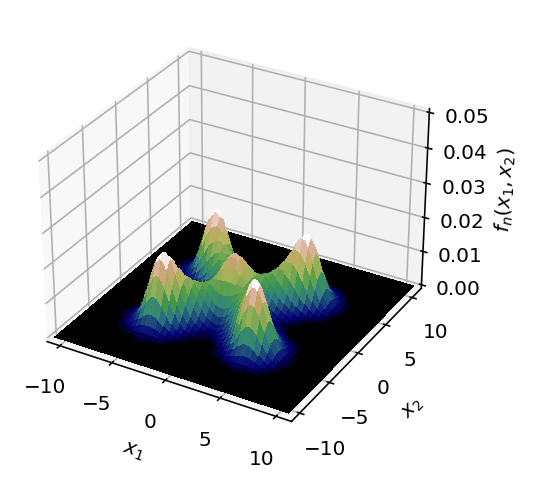
\includegraphics[width=0.8\linewidth]{density.png}
	\caption{A density estimate of the 2 dimensional cross distribution.}
	\label{density_estimate_100GB}
\end{figure}

\section{Results and Scalability}
Results found in Table \ref{table_1TB} and \ref{scale_table_100GB}  were done on clusters using c4.4xlarge (30GB memory, 16 cores) as their worker and driver type. For more details on the compute 
environment see notebooks in \cite{SparkDensityTreeExamples}.
The number of cores used for all results involving 1 TB data sets were 256 cores, or 16 worker nodes.
Table \ref{scale_table_100GB}
contains timings for 100 GB data sets using different number of cores, in order to check the scalability properties
of the library. In the best case, a doubling of the number of cores would halve the run time. Inspecting the Table does not show perfect scaling, but something close to it. The $\overline{\varphi}$ column refers to the count limit used. The maxLeafCount column in Table \ref{depth_1TB} contains the 
maximum data point count found amongst all leaves at the maximal common depth of the leaf-labelling map given in the finestResDepth column. A 70/30 split was applied to create training and validation data sets for the results in Table \ref{table_1TB} and Table \ref{scale_table_100GB}.

\begin{table}[H]
\begin{center}
\begin{tabular}{|c  c  c | c  | c | c | c | c | c |}
	\hline
	$f$ &  $d$ & $n$ &  $\overline{\varphi}$ & $L_1$ Error & Total Time (h:m) \\
	\hline
	Uniform 	& 2  & $6.25$e+$10$ & 100000 & 2.17e-5 & 07:11 \\
	Uniform 	& 10 & $1.25$e+$10$ & 100000 & 3.46e-9 & 00:45 \\
	\hline                 
	\hline
	Cross   	& 2  & $6.25$e+$10$ & 100000 & - & 04:42 \\
	Cross   	& 10 & $1.25$e+$10$ &  20000 & - & 00:46 \\
	\hline
\end{tabular}
\end{center}
\caption{Timings for each density $f$ in dimension $d$ using 1TB of data. In every case the training set were assigned 70\% of the data, with the validation data being assigned the remaining 30\%. No $L_1$ errors for the cross distribution were computed.}
\label{table_1TB}
\end{table}

\begin{table}[H]
\begin{center}
\begin{tabular}{|c  c | c | c |}
	\hline
	$f$ &  $d$ & finestResDepth & maxLeafCount\\
	\hline
	Uniform 	& 2  &  60 & 2  \\
	Uniform 	& 10 &  60 & 6  \\
	\hline                 
	\hline
	Cross   	& 2  &  44 & 3  \\
	Cross   	& 10 &  60 & 5  \\
	\hline
\end{tabular}
\end{center}
\caption{Depths chosen to split down the training and validation data to for the timed runs in Table \ref{table_1TB} by density $f$ and dimension $d$. The maximum number of points found in any leaf is provided in the maxLeafCount column.}
\label{depth_1TB}
\end{table}

Table \ref{breakdown_table_1TB} breaks down the timings of Table \ref{table_1TB}. The first column that stands out is the labelTrain column in which each data point in the training set is transformed into a leaf after which a \textbf{reduceByKey} shuffle operation is applied. Note the difference in time between the 2 dimensional cross and the 2 dimensional uniform. This may simply be due to the uniform
having been run on too few partitions. The second column that stands out is mergeRDD. It is at this point that the reduced leaves are merged up to the count limit, an operation that requires a shuffle and a local
sort of every partition. We chose 16384 partitions as this number of partitions was the first power of 2 that didn't crash at this stage. 
The crashes were most likely due to out of memory errors in the workers.
The last column in the table contains the timings for labelling the validation data and 
the adaptive search for the MDE. The * mark in the 10 dimensional cross case refers to the finest histogram  being the
best performing one, and as such, an early exit was made.
%% New
A column for getCountLimit timings is also provided. The method takes as input
a smallest wanted count limit provided by the user. If no leaf contains a count
exceeding the provided value, the wanted limit can be safely used in the merging
stage and is returned by the method. However, if the limit is exceeded, 
the largest count amongst the leaves is returned instead, as it is the minimum 
viable count limit that can be used in the merging of the leaves. We need to use
the output of this method if we are to be sure that no leaf violates the count limit.
Luckily, the cost of calling the method is small in relation to the shuffling stages.

\begin{table}[htbp]
\begin{center}
\scriptsize{
%\hspace*{-2.4cm}
\begin{tabular}{|c  c  | c | c  | c | c | c |}
	\hline
	$f$ &  $d$ & Hull & labelTrain & getCountLimit & mergeRDD & labelValid \& getMDE \\
	  & & Partitions & Partitions & Partitions & Partitions & Partitions \\
	\hline
	Uniform 	& 2  & 00:06:47 & 04:08:00 & 00:03:25 & 02:53:00 & 00:16:05  \\
	 	        &    & 4096 & 4096 & 4096 & 16384 & 4096  \\
	\hline
	Uniform 	& 10 & 00:06:34 & 00:15:40 & 00:00:45 & 00:19:39 & 00:02:41  \\
	 	        &    & 8192 & 8192 & 8192 & 8192 & 4096 \\
	\hline
	\hline                                                        
	Cross	  	& 2 & 00:07:13 & 01:35:00 & 00:03:01 & 02:22:00 & 00:34:30 \\
	  		&   & 16384 & 16384 & 16384 & 16384 & 4096  \\
	\hline
	Cross  		& 10 & 00:04:22 & 00:13:59 & 00:00:43 & 00:21:03 & 00:06:10*  \\
	 	        &    & 8192 & 8192 & 8192 & 8192 & 4096 \\
	\hline
\end{tabular}
}
\caption{Breakdown of the timings in Table \ref{table_1TB} by density $f$ and dimension $d$. Below every timing is written the number partitions of the data used as input.}
\label{breakdown_table_1TB}
\end{center}
\end{table}

\begin{table}[htbp]
\begin{center}
\begin{tabular}{|c  c  c | c | c | c | c |}
	\hline
	$f$ &  $d$ & $n$ & Cores &  Total Time (h:m:s) \\
	\hline
	Uniform & 2 & $6.25$e+$9$ & 64   & 01:30:08 \\
	Uniform & 2 & $6.25$e+$9$ & 128  & 00:49:34 \\
	Uniform & 2 & $6.25$e+$9$ & 256  & 00:28:23 \\
	\hline
	\hline
	Cross  & 2 & $6.25$e+$9$ & 64    & 01:43:57 \\
	Cross  & 2 & $6.25$e+$9$ & 128   & 01:00:13 \\
	Cross  & 2 & $6.25$e+$9$ & 256   & 00:37:26 \\
	\hline
\end{tabular}
\end{center}
\caption{Timings for the 2 dimensional ($d=2$) cross and uniform density $f$ using 100GB of data with sample size $n$ for various numbers of cores. In every case the training set were assigned 70\% of the data, with the validation data being assigned the remaining 30\%.
The count limit was set to $\overline{\varphi} = 10000$ in every case.}
\label{scale_table_100GB}
\end{table}

A comparison between a Databricks photon accelerated run and a non-accelerated run can be found in Table \ref{photon_1TB}. A driver and 16 Workers of type r6i.2xlarge (64GB memory, 8 cores) were used for
both cases. No perceivable performance boost could be found in the photon accelerated case. 

\begin{table}[htbp]
\begin{center}
\begin{tabular}{|c  c  c  c | c | c  | c | c | c | c |}
	\hline
	$f$ &  $d$ & $n$ & Accelerated & total time (h:m) \\
	\hline
	Cross  	& 2 & $6.25$e+$10$ & yes & 05:21 \\
	\hline
	Cross  	& 2 & $6.25$e+$10$ & no & 04:26 \\
	\hline
\end{tabular}
\end{center}
\caption{Timings for photon acceleration enabled and disabled for the cross density $f$ with dimension $d=2$. }
\label{photon_1TB}
\end{table}

\section{Discussion}

Choosing an appropriate depth is important; going too shallow risks generating leaves exceeding the wanted count limit, while
larger depths entail both an increase in computation time in the labelling stage and greater memory consumption with labels becoming larger in size and the user having to store potentially more unique leaves.
This in turn also hurts the merging and minimum distance estimate stages since the total number of 
bytes being read and shuffled increases.
However, it may not be possible in practice for the user to know what a reasonable depth would be and thus an educated guess has to be made. The memory usage of a leaf at a chosen maximal depth $d$ can be reasoned about as follows.

The underlying structure of a leaf's address or label can be viewed as a 
sequence of bytes in which the bit representing split $d$ is the rightmost bit in the sequence. The second to last split has its bit position found second to last in the sequence, and so on. The 
root bit which is always $1$ is found to the left of the first split's bit. The leftmost bit in the sequence is reserved for the sign bit, which in this case will always be 0, and is due to 
the label being a Java BigInteger. As a small example, we consider a label layout in which 7 splits where made and in each split the left partition was chosen. Theoretically, to represent the label we need 1 bit 
corresponding to the root set to 1, and the following 7 bits set to 0 representing left turns. In practice, the leftmost bit is reserved for a sign bit set to $0$, and thus $9$ bits are required. It follows that the label 
must be represent using 2 bytes with the following layout:
\begin{align*}
	\quad \ \ \text{byte 1} \ \quad &\quad \quad \text{byte 2}\\
	[00000000] &\times [10000000]
\end{align*}
Generalising the above, given a wanted maximal depth of $d$, the size of a (NodeLabel, Count) leaf structure is given below, not counting any underlying pointer memory used.
\begin{align*}
	\bigg\lceil\frac{d + 2}{8}\bigg\rceil + 8 \text{ bytes}
\end{align*}
By constructing the label manually at the bit level inside the labelling routine any unnecessary memory allocation requests could be removed.

The chosen number of partitions when running \textbf{mergeRDD} is also of importance; too few partitions leads to some partitions beings sent more data than they can hold in main memory, and due to the algorithm's
inability to spill data to disk, results in memory errors. The only way to combat this is to choose a larger number of partitions, usually more than the number of cores available, in order for data to be spilled to disk.

The breakdown of timings in Table \ref{breakdown_table_1TB} lets us see how costly the two shuffle operations in the computation of an estimate are. 
Again, the most interesting thing is the large difference in time between the uniform and cross in 2 dimensions for leaf-labelling the training data and applying a \textbf{reduceByKey} operation.
Most likely this is due to the small number of partitions used in the uniform case, which lead to much
larger tasks for the workers. Since each worker was given 30GB of memory and 16 cores,
16 tasks were run in parallel, competing for the resources of the worker. Another interesting observation from the Table is the difference in performance between the
uniform and cross at getMDE, the MDE search stage. The stage starts with the labelling of the validation data, after which we determine the empirical measure of the validation
data over the Scheffé sets within the first iteration's Yatracos class. The first iteration of the search also contains a \textbf{reduceByKey} operation applied on our merged intermediate representation of 
the validation data, which makes consecutive merges of the validation data very cheap. 

The stage also highlights the computational differences in the serial part of the algorithm for when the 
resulting MDE's number of leaves varies. If the unknown density $f$ being estimated is of high complexity or low entropy,
the MDE will usually contain relatively many leaves.
In the case of the cross, the search ended with an estimate containing 596603 leaves, while the uniform with maximal entropy ended with 21 leaves. The cost in the serial part comes from the construction of the
CRP in every iteration being done in a recursive way. The method works well for sets of histograms with significant differences between them, but does not exploit the idea that,
when the finest and coarsest histogram under consideration are close to being equivalent, we can almost create the whole CRP just from only looking at the two estimates. This is explained more in detail
in the next section.

We end the discussion by returning to the theoretical implications of the choice of maximal depth. The finest resolution of leaf labels or addresses for a given sample $(l_1,\dots,l_n)$ is the smallest depth $d$ for which the leaf-labelling map from the sample data points to leaf labels or addresses becomes injective.
This injective mapping of the data points to the leaves that are all at the common maximal depth $d$ creates the coarsest histogram in the collection of all regularly
paved histograms sharing the same root box as the one used in the mapping and 
with leaves of equal depth and counts of 0 and 1.
Thus we can describe arbitrarily complex densities, at least theoretically, by splitting down to this finest resolution and then merge up the leaves to some given limit. Practically, we are of course limited by the machine's memory and computing resources in general.

\section{Further Work}

Many of the performance improvements in this thesis have come from simple optimisations removing unnecessary heap allocations and working directly on bits using bit operations. We suspect that there are still some low hanging 
 optimisations left. The current NodeLabel class wraps an array of bytes representing a leaf's label by two extra classes; a Java BigInteger wrapped by a Scala BigInt. The memory usage of our algorithms could possibly be
reduced if we skipped the NodeLabel and big integer classes altogether, and instead only stored an array of bytes and defined any NodeLabel operations directly using bit operations. This would also remove unnecessary heap allocations made in certain 
methods of the NodeLabel class, such as checking ancestry between NodeLabels, or doing left-right comparisons, both of which are extensively used in stage 3 and 4. 

Some effort would also be well placed in going through the subtree partitioning algorithm to see if there are other ways of doing it, or if a new algorithm would be more suitable. Is there a way of 
doing a cheap initial merge on every partition locally, and then shuffle the data around and doing a final merge such that you can guarantee that the two merges generate a correct result adhering to the count limit?
This would result in less data being shuffled around and might be worth investigating.

In the distributed Scheffé set calculations section we mentioned that a CRP for a given set of histograms may have to store many more leaves than any of the histograms it is based on. The number of leaves will increase quickly
as the difference in size between the coarsest and finest histogram grow. This is due to the fact that the CRP must represent any 0-leaf of the finest histogram that has a non-0-leaf of the coarsest histogram on its path.
If the growth of CRPs do become a problem as we start to construct finer histograms in the merging stage, 
new ways of determining an MDE can be investigated. 
The adaptive search uses a heuristic in order to search the whole path of histograms for a good estimate.
The search range decreases for every iteration until we cannot zoom in on the path any further.
This heuristic is by no means the only way of searching for an estimate, and 
other methods could be explored 
in which you would divide up the path into sectors, and apply the adaptive search within every individual sector. That way you reduce the difference in size between the coarsest and finest histogram used in every adaptive search.

In the construction of the CRP during an iteration of getMDE, we are comparing each histogram estimate with the expanded representation of the finest histogram in the set of histogram estimates under consideration that are coarser than it. Any leaves of the finer histogram (including 0-leaves) that are found within the subtree of a leaf of the coarser histogram must be represented in the finer histogram's expanded representation. Once all estimates have been iterated over, the leaves of the CRP have been determined, and they are exactly those of the expanded representation of the finest histogram.

The issue with this recursive approach is that, when we are comparing almost identical histograms 
only differing by a few leaves, we are still iterating over every histogram's leaves. This works fine
when all histogram's are relatively different, but it entails a great deal of unnecessary computation when
the histograms are almost equivalent, differing only by a few leaves.

What could be done instead is to take an iterative approach in which we are considering all histograms
at once. Suppose that we iterate over all histograms' leaves from left to right. First, note that 
whenever there is equality between two leaves in the coarsest and finest histogram, all histograms
will contain that leaf. Thus, whenever
the two histograms are almost equal in every leaf, we can skip a lot of repetition. Furthermore, 
remember that the reason we care about the CRP is to construct Scheffé sets, but a leaf contained 
in all histograms will not be contained in any Scheffé set, so we could safely ignore such leaves.

The labelling algorithm may also allow for further improvements. 
The current splitting procedure of data points contain a branch for every split, which results in
a lot of branching if the choice of depth to split down to is large. Branches in code can be 
relatively costly in comparison to arithmetical operations, and making an effort in writing the
code in a branchless fashion may increase performance. Removing branches in our case would entail
finding an efficient mapping from any point $p$ to its corresponding bit value for any given depth.
We give an example. Given a box hull $(a,b)$ consisting of two vectors where $a$ 
contains the minimum values for each dimension and $b$ the maximal ones, one such mapping is: 
\begin{align*}
	\bigg\lfloor \bigg(\ \frac{p_i - a_i}{b_i - a_i} - \epsilon \bigg\lfloor\frac{p_i - a_i}{b_i - a_i}\bigg\rfloor\ \bigg) \cdot n_\text{cells} \bigg\rfloor \ \text{mod}\  2 \enspace,
\end{align*}
where $i$ denotes the current dimension we are splitting, and $n_\text{cells}$ refers to the number of cells 
the split will create in the given dimension. It  follows that any point in the first box will be mapped to $0$, the second box to
$1$, the third to $0$, and so on. Note that $\epsilon$ is only relevant for the special case in which we are mapping the point with the maximum value in the given dimension. Then $p_i$ is equivalent to $b_i$ and it would follow that
the point would be incorrectly mapped to $0$ if we had not translated $p_i$ by some small value. Thus $\epsilon$ must be small enough such that it won't change the correct labelling, 
but large enough for $p_i$ to be smaller than $b_i$. Since any mapping similar to this introduces
more floating point arithmetic, it is bound to become unstable after enough splitting. One would have to prove for which ranges any such mapping produces correct results,
and if more splitting is required than what would be considered safe, it would be easy to fall back to the original routine. 

\chapter*{Support}
This project was partly supported by \textit{Databricks University Alliance} with infrastructure credits from AWS, and a grant from Wallenberg AI, Autonomous Systems and Software Program funded by Knut and Alice Wallenberg Foundation to Raazesh Sainudiin, Department of Mathematics, Uppsala University, Sweden.
It was also supported by Combient Mix AB through 2023 summer internship in Data Engineering Sciences to Axel Sandstedt at Combient Competence Center for Mathematical Data Engineering Sciences, Department of Mathematics, Uppsala University, Sweden. 


\begingroup
	\begin{thebibliography}{9}
		\bibitem{CMDE}
			Luc Devroye \& Gábor Lugosi.
			\textit{Combinatorial Methods in Density Estimation}.
			Springer-Verlag, New York, 2001.
		\bibitem{Consistency}
			Gábor Lugosi \& Andrew Nobel.
			Consistency of Data-Driven Histogram Methods for Density Estimation and Classification.
			\textit{The annals of Statistics}, 24(2):687-706, 1996.
		\bibitem{Pattern}
			Luc Devroye, László Györfi \& Gábor Lugosi.
			A Probabilitstic Theory of Pattern Recognition
			Springer-Verlag, New York, 1996.
		\bibitem{Martingales}
			David Williams.
			\textit{Probability with Martingales}
			Cambridge University Press, 1991.
		\bibitem{Mapped Regular Pavings}
			Jennifer Harlow, Raazesh Sainudiin \& Warwick Tucker.
			Mapped Regular Pavings.
			\textit{Reliable Computing}, 16, 252-282, 2012.
		\bibitem{MDE}
			Raazesh Sainudiin \& Gloria Teng.
			Minimum distance histograms with universal performance guarantees.
			\textit{Japanese Journal of Statistics and Data Science}, 2:507-527, 2019.
		\bibitem{Scalable Multivariate Histograms}
			Raazesh Sainudiin, Warwick Tucker \& Tilo Wiklund.
			Scalable Multivariate Histograms.
			https://arxiv.org/abs/2012.14847, 2020.
		\bibitem{Scalable Algorithms}
			Johannes Graner.
			Scalable Algorithms in Nonparametric Computational Statistics.
			http://urn.kb.se/resolve?urn=urn:nbn:se:uu:diva-488518, 2022.
		\bibitem{Algorithm Design}
			Jon Kleinberg \& Éva Tardos.
			\textit{Algorithm Design}.
			Pearson, 2005.
		\bibitem{The Design of Approximation Algorithms}
			David P. Williamson \& David B. Shmoys.
			\textit{The Design of Approximation Algorithms}.
			Cambridge University Press, first edition, 2011.
		\bibitem{clrs}
		Thomas H. Cormen, Charles E. Leiserson, Ronald L. Rivest \& Clifford Stein.
			\textit{Introduction to Algorithms}.
			The MIT Press, fourth edition, 2022.
		\bibitem{L-algorithm}
			Kim-Hung Li.
			Reservoir-Sampling Algorithms of Time Complexity O(n(1+log(N/m))).
			\textit{ACM Transactions on Mathematical Software}, 20(4):481-493, 1994
		\bibitem{ks}
                Tarn Duong, Matt Wand, Jose Chacon \& Artur Gramacki.
			ks: Kernel Smoothing.
			https://cran.r-project.org/package=ks, 2023
		\bibitem{SparkDensityTree}
			Axel Sandstedt, Johannes Graner, Tilo Wiklund \& Raazesh Sainudiin.
    {SparkDensityTree: An Apache Spark library for scalable density estimation, anomaly detection and conditional density regression with universal performance guarantees through distributed sparse binary trees (Version 1.0) [Computer software].} https://github.com/lamastex/SparkDensityTree, 2023
	\bibitem{SparkDensityTreeExamples}
		Axel Sandstedt, Johannes Graner, Tilo Wiklund \& Raazesh Sainudiin.
	{SparkDensityTree-examples: User-guide with examples for SparkDensityTree library (Version 1.0) [Computer software].} https://github.com/lamastex/SparkDensityTree-examples, 2023
		\bibitem{spark sort}
  Zaharia, M., Xin, R. S., Wendell, P., Das, T., Armbrust, M., Dave, A., Meng, X., Rosen, J., Venkataraman, S., Franklin, M. J., Ghodsi, A., Gonzalez, J., Shenker, S. \& Stoica, I. (2016). 
  Apache Spark: A Unified Engine for Big Data Processing. Communications of the ACM, 59, 56--65. doi: 10.1145/2934664.
  \end{thebibliography}
\endgroup

%%%%%%%%%%%%%%%%
%\chapter{Appendix}
\appendix
\renewcommand\chaptername{Appendix}
\chapter{Additional Results}
In this Appendix, we present additional results using the spark implementation found in \cite{SparkDensityTree} that help demonstrate other aspects of the estimator, including how it scales with dimension and the number of workers on a family of densities with different sample sizes and dimensions.

Timings were done on Databricks using runtime environment 12.2 LTS, which includes Apache Spark 3.3.2, Scala 2.12. 
The specifications of the cluster for the Gaussian case is
9 e2-highmem-2 (16GB memory, 2 cores) cpu workers and an e2-highmem-2 cpu driver, and in the Uniform case 4 e2-standard-4 cpu workers (16 GB memory, 4 cores) and an e2-standard-4 cpu driver. 
No autoscaling of workers was used and no specific java virtual machine arguments were given. The validation size were in every case half as large as the given training size $n$. 

Recall the four stages of our minimum density estimator (Section~\ref{S:4Stages}). Table \ref{shared_table} contains timings for stages 1, 2 and 4 for various cases. The parameter $\overline{\varphi}$ refers to the count limit used in each case at stage 3. 
We note the long runtimes for calculating the box hull and labelling each leaf in the 1000D Uniform case. In stage 2, the chosen depths for the Gaussian 1D, 2D, 5D and 100D cases were 21, 42, 70 and 700, respectively. The depths for the Uniform cases of $n=10^7$ and $n=10^8$ were chosen to be 47 and 54, respectively.

Table \ref{rdd_ds_table} shows the timings for both the old (Spark dataset or DS) and new (Spark RDD) version of the backtracking or merging problem in stage 3. The mergeDS/mergeRDD timing refers to the time it 
took for the two methods to fetch labelled leaves from disk and merge them up to the given count limit in stage 3. 
In the subtree partitioning method the sample size hint, or roughly the number of data points sampled 
for each new subtree partition, was set to 1000 for all cases (see the sampling subsection in Section~\ref{SubtreePartitioning} for more details). Note that 
in \textbf{mergeRDD}, the number of partitions in some cases exceed the number of total cores, something which may be needed in order for the algorithm to be able to spill to disk
and not run out of memory. 

Table \ref{rdd_table} Shows the final timings and $L_1$ errors for varying cases. The timing refers to the total time across all stages, assuming that \textbf{mergeRDD} was used.
Note the * symbol in the 5D and 100D Gaussian entries; it indicates that stage 4 exited early because the finest histogram was found to be the best performing one in the first iteration, and thus
no more iterations were made, which results in a shorter runtime. 
Such an early exit means that count limit is too high as we have not started from a fine enough histogram partition so that the optimally smoothed minimum distance estimate lies among histograms with coarser partitions than the starting one. 
Also, no $L_1$ errors were calculated for the multivariate Gaussians due to difficulties in accurate high-dimensional quadrature (\cite{Scalable Algorithms}, p. 38).


\begin{sidewaystable}[htbp]
\begin{center}
\begin{tabular}{|c  c  c | c | c | c | c |}
	\hline
	Distribution &  Dimensions &  $n$ & $\overline{\varphi}$ & Hull (h:m:s) & Labelling (h:m:s) & getMDE (h:m:s) \\
	\hline
	Uniform	& 1  & 		$10^7$ & 1000 &  00:00:04  & 00:00:39 & 00:00:17 \\
	Uniform	& 10  & 	$10^7$ & 1000 &  00:00:19  & 00:00:57 & 00:00:16 \\
	Uniform	& 100  & 	$10^7$ & 1000 &  00:01:21  & 00:01:32 & 00:00:16 \\
	Uniform	& 1000  & 	$10^7$ & 1000 &  00:10:19  & 00:03:37 & 00:00:34 \\
	\hline
	Uniform & 1  & 		$10^8$ & 10000 & 00:00:56  & 00:08:12 & 00:01:35  \\
	Uniform & 10  & 	$10^8$ & 10000 & 00:01:09  & 00:07:27 & 00:01:36  \\
	Uniform & 100  & 	$10^8$ & 10000 & 00:10:21  & 00:08:35 & 00:01:55  \\
	Uniform & 1000  & 	$10^8$ & 10000 & 01:23:00  & 00:16:31 & 00:02:16  \\
	\hline
	\hline
	Gaussian  & 1  & 	$10^7$ & 1000 &  00:00:08 &  00:00:36 & 00:00:17   \\
	Gaussian  & 2  & 	$10^7$ & 1000 &  00:00:07 &  00:00:41 & 00:00:40   \\
	Gaussian  & 5  & 	$10^7$ & 1000 &  00:00:07 &  00:00:39 & 00:00:17*  \\
	\hline
	Gaussian  & 1  & 	$10^8$ & 10000 & 00:01:07 &  00:02:25 & 00:00:17  \\
	Gaussian  & 2  & 	$10^8$ & 10000 & 00:01:08 &  00:06:27 & 00:01:32  \\
	Gaussian  & 5  & 	$10^8$ & 10000 & 00:01:09 &  00:06:37 & 00:01:09* \\
	Gaussian  & 100  & 	$10^8$ & 3000 &  00:11:38 &  00:15:10 & 00:01:56* \\
	\hline
\end{tabular}
\end{center}
\caption{Timings for the shared parts of the previous and new algorithm.}
\label{shared_table}
\end{sidewaystable}

\begin{sidewaystable}[htbp]
\begin{center}
\begin{tabular}{|c  c  c | c | c | c | c | c |}
	\hline
	Distribution &  Dimensions &  $n$ & $\overline{\varphi}$ & mergeDS (h:m:s) & mergeRDD (h:m:s) & subtreePartitions \\
	\hline
	Uniform	& 1  & 		$10^7$ & 1000  & 00:01:39 & 00:00:25 &  36 \\
	Uniform	& 10  & 	$10^7$ & 1000  & 00:02:03 & 00:00:25 &  36 \\
	Uniform	& 100  & 	$10^7$ & 1000  & 00:01:53 & 00:00:25 &  36 \\
	Uniform	& 1000  & 	$10^7$ & 1000  & 00:01:35 & 00:00:23 &  36 \\
	\hline
	Uniform & 1  & 		$10^8$ & 10000 & 00:08:38 & 00:04:48 &  128 \\
	Uniform & 10  & 	$10^8$ & 10000 & 00:08:11 & 00:04:50 &  128 \\
	Uniform & 100  & 	$10^8$ & 10000 & 00:07:52 & 00:04:00 &  128 \\
	Uniform & 1000  & 	$10^8$ & 10000 & 00:09:01 & 00:04:00 &  128 \\
	\hline
	\hline
	Gaussian  & 1  & 	$10^7$ & 1000  & 00:02:08 & 00:00:07 & 18 \\
	Gaussian  & 2  & 	$10^7$ & 1000  & 00:02:12 & 00:00:31 & 18	\\
	Gaussian  & 5  & 	$10^7$ & 1000  & 00:02:26 & 00:00:34 & 72\\
	\hline
	Gaussian  & 1  & 	$10^8$ & 10000 & 00:01:40 & 00:00:08 & 18\\
	Gaussian  & 2  & 	$10^8$ & 10000 & 00:05:41 & 00:05:05 & 72\\
	Gaussian  & 5  & 	$10^8$ & 10000 & 00:09:41 & 00:05:02 & 128\\
	Gaussian  & 100  & 	$10^8$ & 3000  & - 	  & 00:08:03 & 1024\\
	\hline
\end{tabular}
\end{center}
\caption{Timings for the merging stage in the new (RDD) and old (DS) version.}
\label{rdd_ds_table}
\end{sidewaystable}

\begin{table}[htbp]
\begin{center}
\begin{tabular}{|c  c  c | c | c |}
	\hline
	Distribution &  Dimensions &  $n$ & $L_1$ Error & Total Time (h:m:s)\\
	\hline
	Uniform	& 1  & 		$10^7$ & 1.11e-3   &   00:01:25 \\
	Uniform	& 10  & 	$10^7$ & 6.86e-4   &   00:01:57 \\
	Uniform	& 100  & 	$10^7$ & 3.15e-5   &   00:03:34 \\
	Uniform	& 1000  & 	$10^7$ & 3.94e-4   &   00:14:53 \\
	\hline                                   
	Uniform & 1  & 		$10^8$  & 1.54e-3  &   00:15:31 \\
	Uniform & 10  & 	$10^8$  & 4.05e-3  &   00:15:02 \\
	Uniform & 100  & 	$10^8$  & 2.68e-6  &   00:24:51 \\
	Uniform & 1000  & 	$10^8$  & 2.64e-5  &   01:45:47 \\
	\hline
	\hline
	Gaussian  & 1  & 	$10^7$ & 5.94e-3 &    00:01:08   \\
	Gaussian  & 2  & 	$10^7$ & - 	 &    00:01:59   \\
	Gaussian  & 5  & 	$10^7$ & - 	 &    00:01:37*     \\
	\hline
	Gaussian  & 1  & 	$10^8$ & 3.03e-3 &    00:03:57   \\
	Gaussian  & 2  & 	$10^8$ & - 	 &    00:14:12  \\
	Gaussian  & 5  & 	$10^8$ & - 	 &    00:13:57* \\
	Gaussian  & 100  & 	$10^8$ & - 	 &    00:36:47* \\
	\hline
\end{tabular}
\end{center}
\caption{Final timings for the whole pipeline of stages for the new RDD based algorithm, excluding the time it took to generate any raw data.}
\label{rdd_table}
\end{table}

\section{Scaling Computation}
Table \ref{scale_table} and Figure \ref{scaling_plot} show how \textbf{mergeRDD} performs as the number of workers increase. Timings were taken for the Gaussian 5D case using $10^8$ data points with the usual sample size hint of 1000. 
The time taken roughly halves for each doubling in the number of workers, with a total reduction in time by 89\% between $1$ and $16$ workers.
\begin{table}[htbp]
\begin{center}
\begin{tabular}{|c  c  c | c | c  | c | c | c |}
	\hline
	$f$ &  $d$ & $n$ & Partitions & Workers & $\overline{\varphi}$  & mergeRDD (s) \\
	\hline
	Gaussian  & 5 & $10^8$ & 128 & 1   & 10000 & 1147 \\
	Gaussian  & 5 & $10^8$ & 128 & 2   & 10000 & 596 \\
	Gaussian  & 5 & $10^8$ & 128 & 4   & 10000 & 343 \\
	Gaussian  & 5 & $10^8$ & 128 & 8   & 10000 & 186 \\
	Gaussian  & 5 & $10^8$ & 128 & 16  & 10000 & 130 \\
	\hline
\end{tabular}
\end{center}
\caption{Timings for powers of $2$ number of workers given a sample of $10^8$ points from a standard 5D Gaussian.}
\label{scale_table}
\end{table}

\begin{figure}[htbp]
\begin{center}
	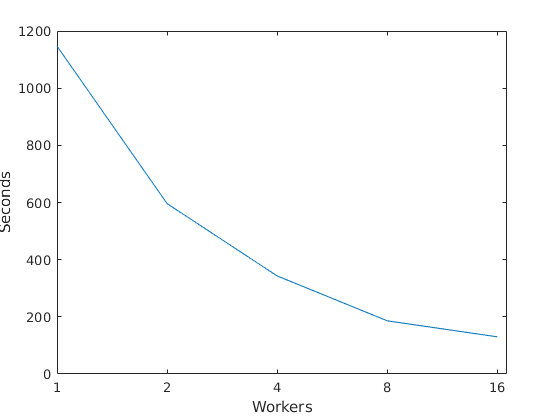
\includegraphics[scale=0.550]{scalePlot.png}
	\caption{Plot of merge timings for the 5D standard Gaussian case with $n=10^8$ points and an increasing number of workers.}
	\label{scaling_plot}
 \end{center}
\end{figure}


\section{Performance of multivariate Gaussian estimates}
%% TODO needs to be rewritten much closer to page 38/38 of
% https://uu.diva-portal.org/smash/get/diva2:1711540/FULLTEXT01.pdf
To measure the performance of the multivariate Gaussian estimates we verify how well the estimator performs
as a discriminator. The discrimination property is inspected by constructing an estimate from the
standard Gaussian, and an estimate from the translated standard Gaussian $N(\overline{\delta}(c), I)$ where each entry of $\overline{\delta}(c)$ is set to $\frac{c}{\sqrt{\text{dimensions}}}$. The two estimates 
are constructed using training sets of size $n=10^8$ and validation sets that are half the size of the training sets. two additional samples of size $n=10^6$ are then generated from the underlying
distributions, and for every sampled data point, it is determined which of the two estimates achieves the
larger density at the point's location.

In Table \ref{confusion_table} we find various confusion matrices corresponding to distributions shifted
further and further away from the standard Gaussian for different dimensions. 

\begin{sidewaystable}[htbp]
\begin{center}
\begin{tabular}{| c c || c c || c c |}
	\hline
	& 2D Gaussian & & 5D Gaussian & & 100D Gaussian \\
	\hline
	\hline
	$\delta \sqrt{2}$ & Confusion Matrix & $\delta \sqrt{5}$ & Confusion Matrix & $\delta \sqrt{100}$ & Confusion Matrix \\
	\hline
	$1 \sqrt{2}$ 	& $\begin{matrix} \text{TP: }34.5 & \text{FN: } 15.5 \\ \text{FP: }15.5 & \text{TN: }34.5 \end{matrix}$ &
	$1 \sqrt{5}$ 	& $\begin{matrix} \text{TP: }33.1 & \text{FN: } 16.9 \\ \text{FP: }16.6 & \text{TN: }33.4 \end{matrix}$ &
	$10 \sqrt{100}$ & $\begin{matrix} \text{TP: }23.9 & \text{FN: } 26.1 \\ \text{FP: }14.6 & \text{TN: }35.4 \end{matrix}$\\ 
	\hline
	$2 \sqrt{2}$ 	& $\begin{matrix} \text{TP: }42.0 & \text{FN: } 8.0 \\ \text{FP: }7.9 & \text{TN: }42.1 \end{matrix}$ &
	$2 \sqrt{5}$ 	& $\begin{matrix} \text{TP: }41.2 & \text{FN: } 8.8 \\ \text{FP: } 8.7 & \text{TN: } 41.3 \end{matrix}$ &
	$20 \sqrt{100}$ & $\begin{matrix} \text{TP: }37.8 & \text{FN: } 12.2 \\ \text{FP: }10.5 & \text{TN: }39.5 \end{matrix}$\\ 
	\hline
	$3 \sqrt{2}$ 	& $\begin{matrix} \text{TP: }46.6 & \text{FN: } 3.4 \\ \text{FP: }3.4 & \text{TN: }46.6 \end{matrix}$ &
	$3 \sqrt{5}$ 	& $\begin{matrix} \text{TP: }46.2 & \text{FN: } 3.8 \\ \text{FP: } 3.9 & \text{TN: }46.1 \end{matrix}$ &
	$30 \sqrt{100}$ & $\begin{matrix} \text{TP: }32.7 & \text{FN: } 17.3 \\ \text{FP: }8.1 & \text{TN: }41.9 \end{matrix}$\\ 
	\hline
	$5 \sqrt{2}$ 	& $\begin{matrix} \text{TP: }49.7 & \text{FN: } 0.3 \\ \text{FP: }0.3 & \text{TN: }49.7 \end{matrix}$ &
	$5 \sqrt{5}$ 	& $\begin{matrix} \text{TP: }49.5 & \text{FN: } 0.5 \\ \text{FP: }0.5 & \text{TN: }49.5 \end{matrix}$ &
	$50 \sqrt{100}$ & $\begin{matrix} \text{TP: }50.0 & \text{FN: } 0.0 \\  \text{FP: }0.0  & \text{TN: }50.0 \end{matrix}$\\ 
	\hline
\end{tabular}
\end{center}
\caption{Confusion matrices for the 2D, 5D and 100D Gaussian estimates with training set size $n=10^8$.
	The same estimate was continuously tried against newly generated estimates from a translated standard Gaussian distribution. $\delta \sqrt{\text{dimensions}}$
	refers to the translation applied to the transformed distribution where each axis is translated by $\frac{\delta}{\sqrt{\text{dimensions}}}$.}
\label{confusion_table}
\end{sidewaystable}


\end{document}

